\chapter{Computational Results}\label{chap:results}

This chapter shows the results from testing all the shortest path algorithms detailed in Chapter~\ref{chap:solvingspp} using the specific implementation described in the previous chapter.

\todoin[inline]{Convergence and Rel gap! 1e-6 for all networks}

Implemented by Olga, the co-supervisor.
Note the traffic assignment algorithms have already been implemented by the co-supervisor of this report in a Object Oriented C++ program.
The programs includes Frank-Wolfe, Path Equilibration,
label correcting algorithm and many more.

The results are generated from using the g++ compiler using the -O3 optimise for speed option on Ubuntu 12.04 operating system, which has a Intel Core i5-3317U CPU with 3.8GiB RAM.

\section{Problem Data and Result Explanation}
The problem data for solving the TA problems are retrieved from Transportation Network Test Problems \citep{ProblemData}.
Table~\ref{table:problemdata} shows the data that are going to be tested with,
where the network name, numbers nodes, traffic analysis, origin-destination (OD) pairs and edges are given.
\begin{table}[H]
    \centering
    \begin{tabular}{lrrrr} \toprule
        Network & Nodes & Zones & OD pairs & Edges \\ \cmidrule(lr){1-5}
        %SiouxFalls    & 24   & 24  & 528   & 76   \\
        Anaheim       & 416  & 38  & 1406  & 914  \\
        Barcelona     & 1020 & 110 & 7922  & 2522 \\
        Winnipeg      & 1052 & 147 & 4344  & 2836 \\
        ChicagoSketch & 933  & 387 & 93135 & 2950 \\ \bottomrule
    \end{tabular}
    \caption{Network Problem Data}
    \label{table:problemdata}
\end{table}
By examining the network problem data,
we can see that the number of OD pairs increase
significantly respect to the number of zone nodes,
this is important because it indicates how many point to point SPPs need to be solved for each iteration of the PE method.
We can also roughly tell that these networks are very sparse;
for a complete graph (every node is connected to every other node) of 1000 nodes have 499500 edges ($n(n-1)/2$),
but the larger networks in our problem data only have about 0.4\% to 0.6\% of edges in the corresponding complete graph. 
Analysing the graph shows the degree of any vertex in the graph is no more than 5.
This information is useful for choosing the best algorithm and data structure.

The correctness of the final shortest path trees are checked by comparing to the label correcting algorithm that is implemented by the co-supervisor of this project, which is guaranteed to be correct.

\section{Discussion of Computational Results}
\begin{comment}
In Table~\ref{table:boostresult} and Table~\ref{table:allresults} we present the running times for a complete run of the Traffic Assignment Path Equilibration method.

Table~\ref{table:boostresult} shows the performance of the Dijkstra's algorithm and the A* search algorithm using the 6 variants of the Heap implementations from the Boost library on the ChicagoSketch network.
The numbers of iterations (ITERS)
and total run time (seconds) of each algorithm took is shown.

\begin{table}[H]
    \centering
    \begin{tabular}{c c c c } \toprule
        Algorithm & Heap & ITERS & Time (sec)\\
        \cmidrule(lr){1-1}
        \cmidrule(lr){2-2}
        \cmidrule(lr){3-3}
        \cmidrule(lr){4-4}
        \multirow{6}{*}{Dijkstra} & Fibonacci & \multirow{6}{*}{25}
             & 155.14 \\
        &    Binary   & & 130.22 \\
        &    Ternary  & & 155.34 \\
        &    Skew     & & 120.45 \\
        &    Pairing  & & 140.55 \\
        &    Binomial & & 369.10 \\
        \cmidrule(lr){1-1}
        \cmidrule(lr){2-2}
        \cmidrule(lr){3-3}
        \cmidrule(lr){4-4}
        \multirow{6}{*}{A*} & Fibonacci & \multirow{6}{*}{26}
                & 31.27 \\
        &    Binary  &&  28.00 \\
        &    Ternary &&  34.31 \\
        &    Skew    &&  25.94 \\
        &    Pairing &&  27.93 \\
        &    Binomial&&  59.76 \\
        \bottomrule
    \end{tabular}
    \caption{Performance of Dijkstra's algorithm and A* search algorithm using 6 variants of the Heap implementation on the ChicagoSketch network. }
    \label{table:boostresult}
\end{table}
\end{comment}

Figure~\ref{fig:pq_runtime2} and~\ref{fig:pq_runtime} shows the performance of Dijkstra's algorithm on both Winnipeg and ChicagoSketch network using priority queue implementations from the C++ Boost library and the Standard Template Library.

On both networks, the Heap implementation from the C++ Standard Template Library out performs all other implementations.
And the Fibonacci Heap does not have the promised runtime behaviour described in Section~\ref{sec:pq_implementation}.
What is interesting is that for the Heaps with $O(\log(N))$ behaviour, their run time vary a lot, especially for the Binomial Heap.

\begin{figure}[H]
    \centering
    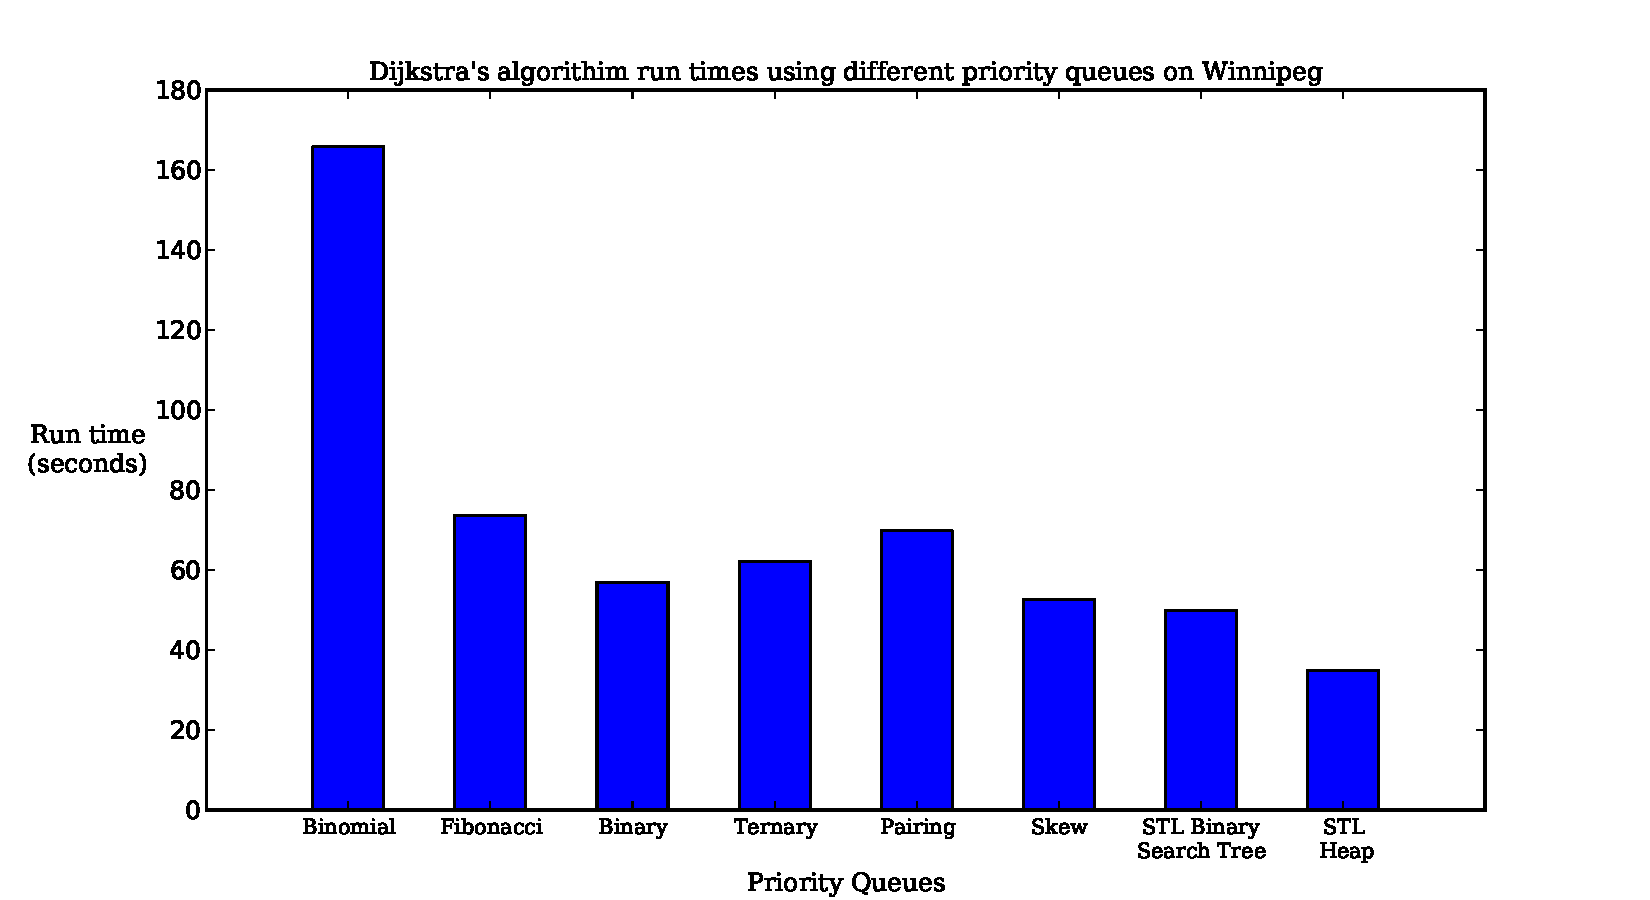
\includegraphics[width=\textwidth]{img/pq_runtime2}
    \caption{Dijkstra's algorithm run times using different priority queues on Winnipeg}
    \label{fig:pq_runtime2}
\end{figure}

\begin{figure}[H]
    \centering
    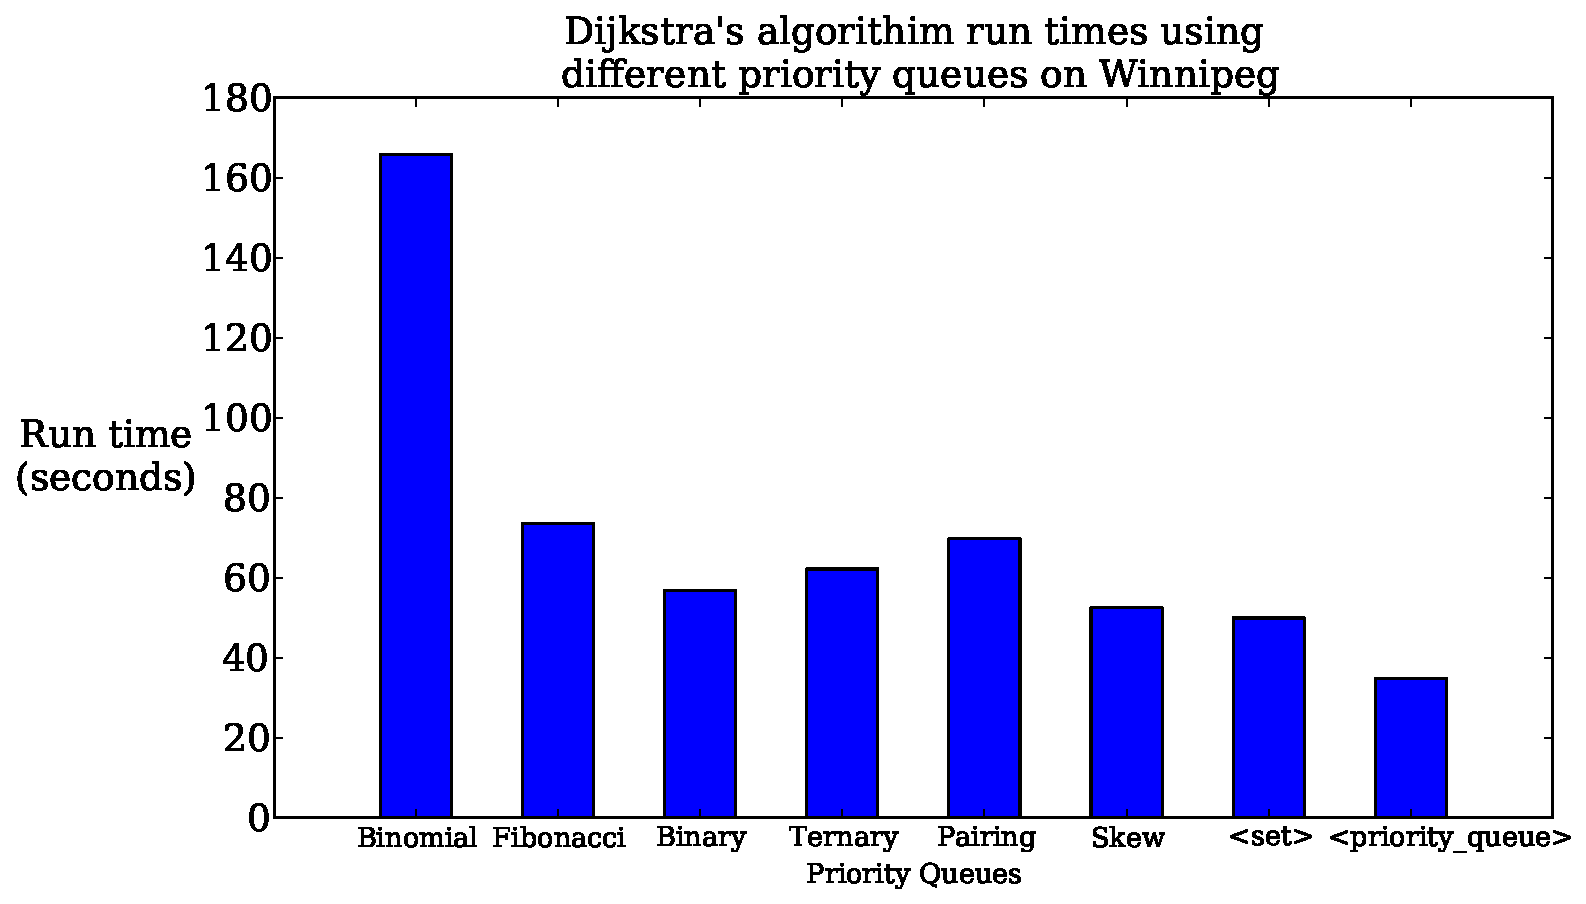
\includegraphics[width=\textwidth]{img/pq_runtime}
    \caption{Dijkstra's algorithm run times using different priority queues on ChicagoSketch}
    \label{fig:pq_runtime}
\end{figure}

Figure~\ref{fig:allresults} shows the performance of each of the algorithms
\begin{itemize}
    \item label correcting Bellman-Ford,
    %\item one source Dijkstra (1S-D),
    \item point to point Dijkstra using heap from C++ standard library,
    \item point to point Dijkstra using binary search tree,
    \item bidirectional Dijkstra,
    \item A* search,
    \item bidirectional A* search,
\end{itemize}
used on each of the networks shown in Table~\ref{table:problemdata}.
%The numbers of iterations (ITERS) each algorithm took,
\begin{figure}[H]
    \centering
    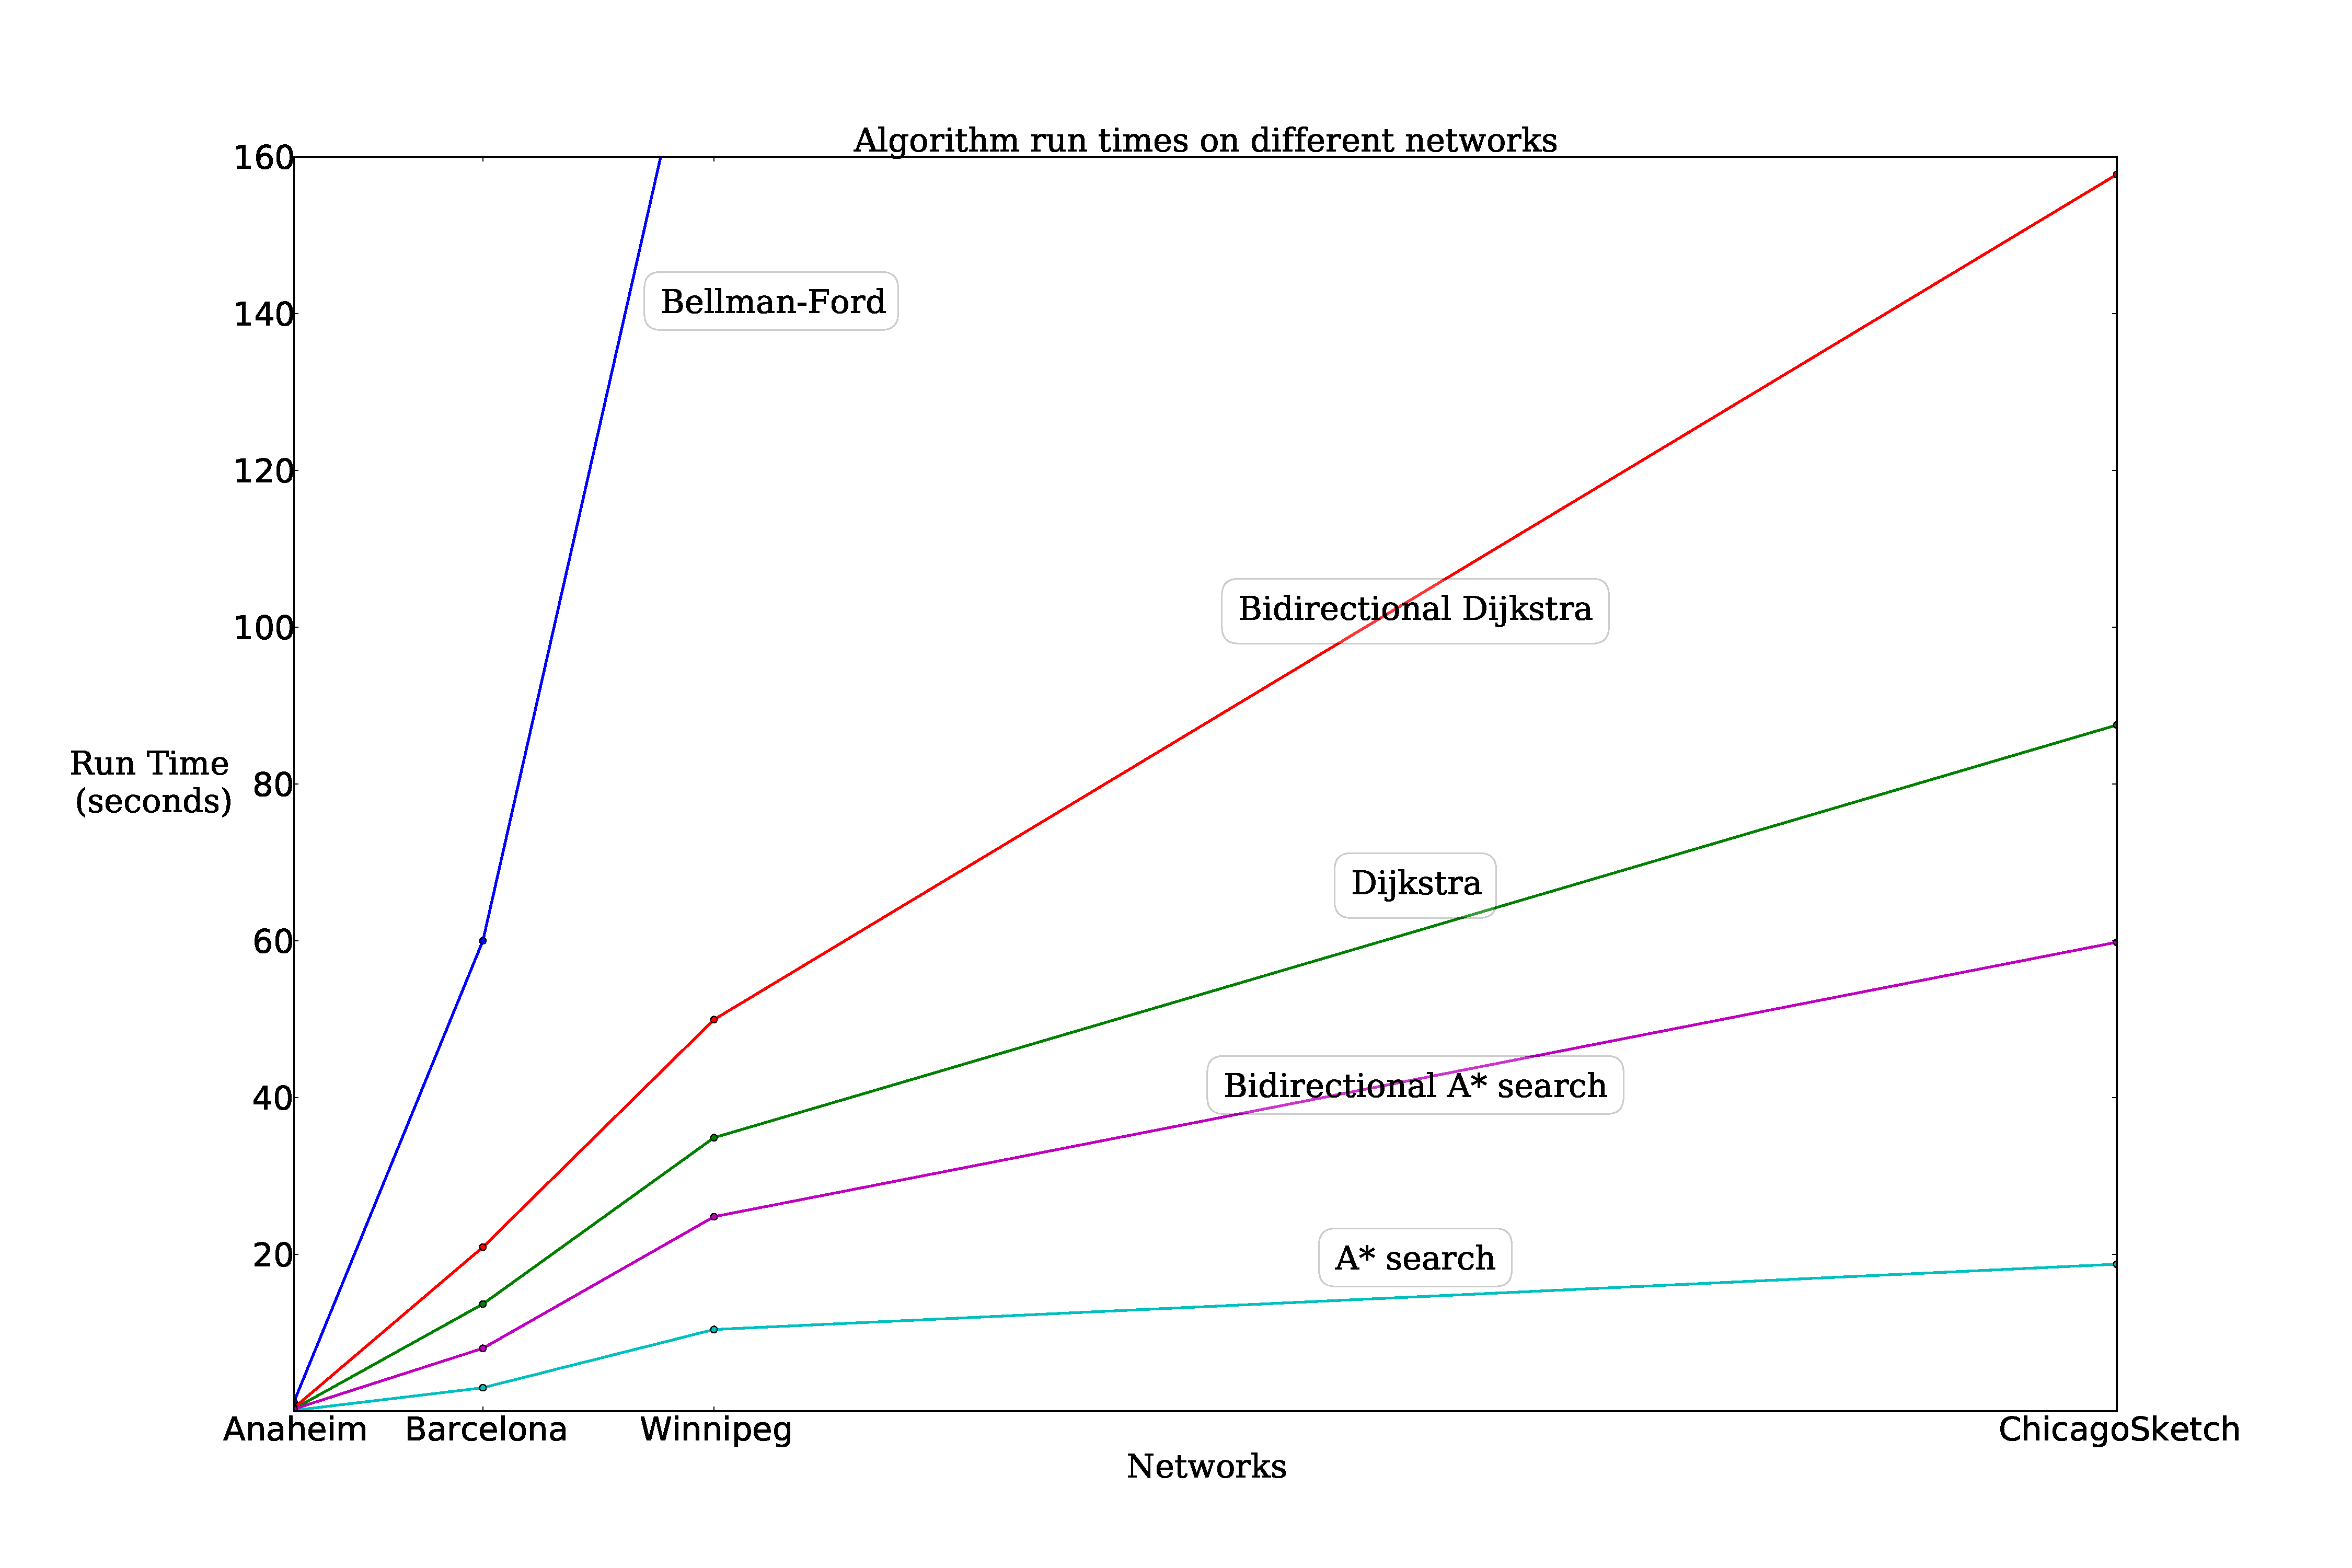
\includegraphics[width=\textwidth]{img/runtime}
    \caption{Run time performances of different algorithms on different networks}
    \label{fig:allresults}
\end{figure}

Now we investigate the reason for the run time behaviours of the shortest path algorithms shown in Figure~\ref{fig:allresults}.
Figure~\ref{fig:long_sptree} shows the shortest path trees of the point-to-point algorithms, where the origin and destination node is placed on the opposite side of the ChicagoSketch network.
It can be seen that Dijkstra's algorithm scans the entire network;
the Bidirectional Dijkstra scans almost the whole network but with a few nodes left out;
The Bidirectional A* search scans a slightly larger region near the origin and destination nodes;
and the A* search only scans a few nodes along the shortest path.
The behaviour of the algorithms is shown further in Figure~\ref{fig:short_sptree},
where the origin and destination is placed close to each other.
The Dijkstra and Bidirectional Dijkstra algorithm need to scan many nodes before termination;
And the A* and Bidirectional A* search only scan a small portion of network,
and they do not scan the area behind the origin and destination node.

The run time of the shortest path algorithms are heavily dependent on the number of nodes they scan.
The process of scanning a node consists of placing the node into a priority queue, taking it out sometime later, and check all its out going arcs.
So cumulatively the less nodes an algorithm scans the faster it runs.
And by examining Figure~\ref{fig:long_sptree} and Figure~\ref{fig:short_sptree},
it is obvious to see A* search is the fastest.

\begin{figure}
    \centering
    \begin{subfigure}{.5\textwidth}
        \centering
        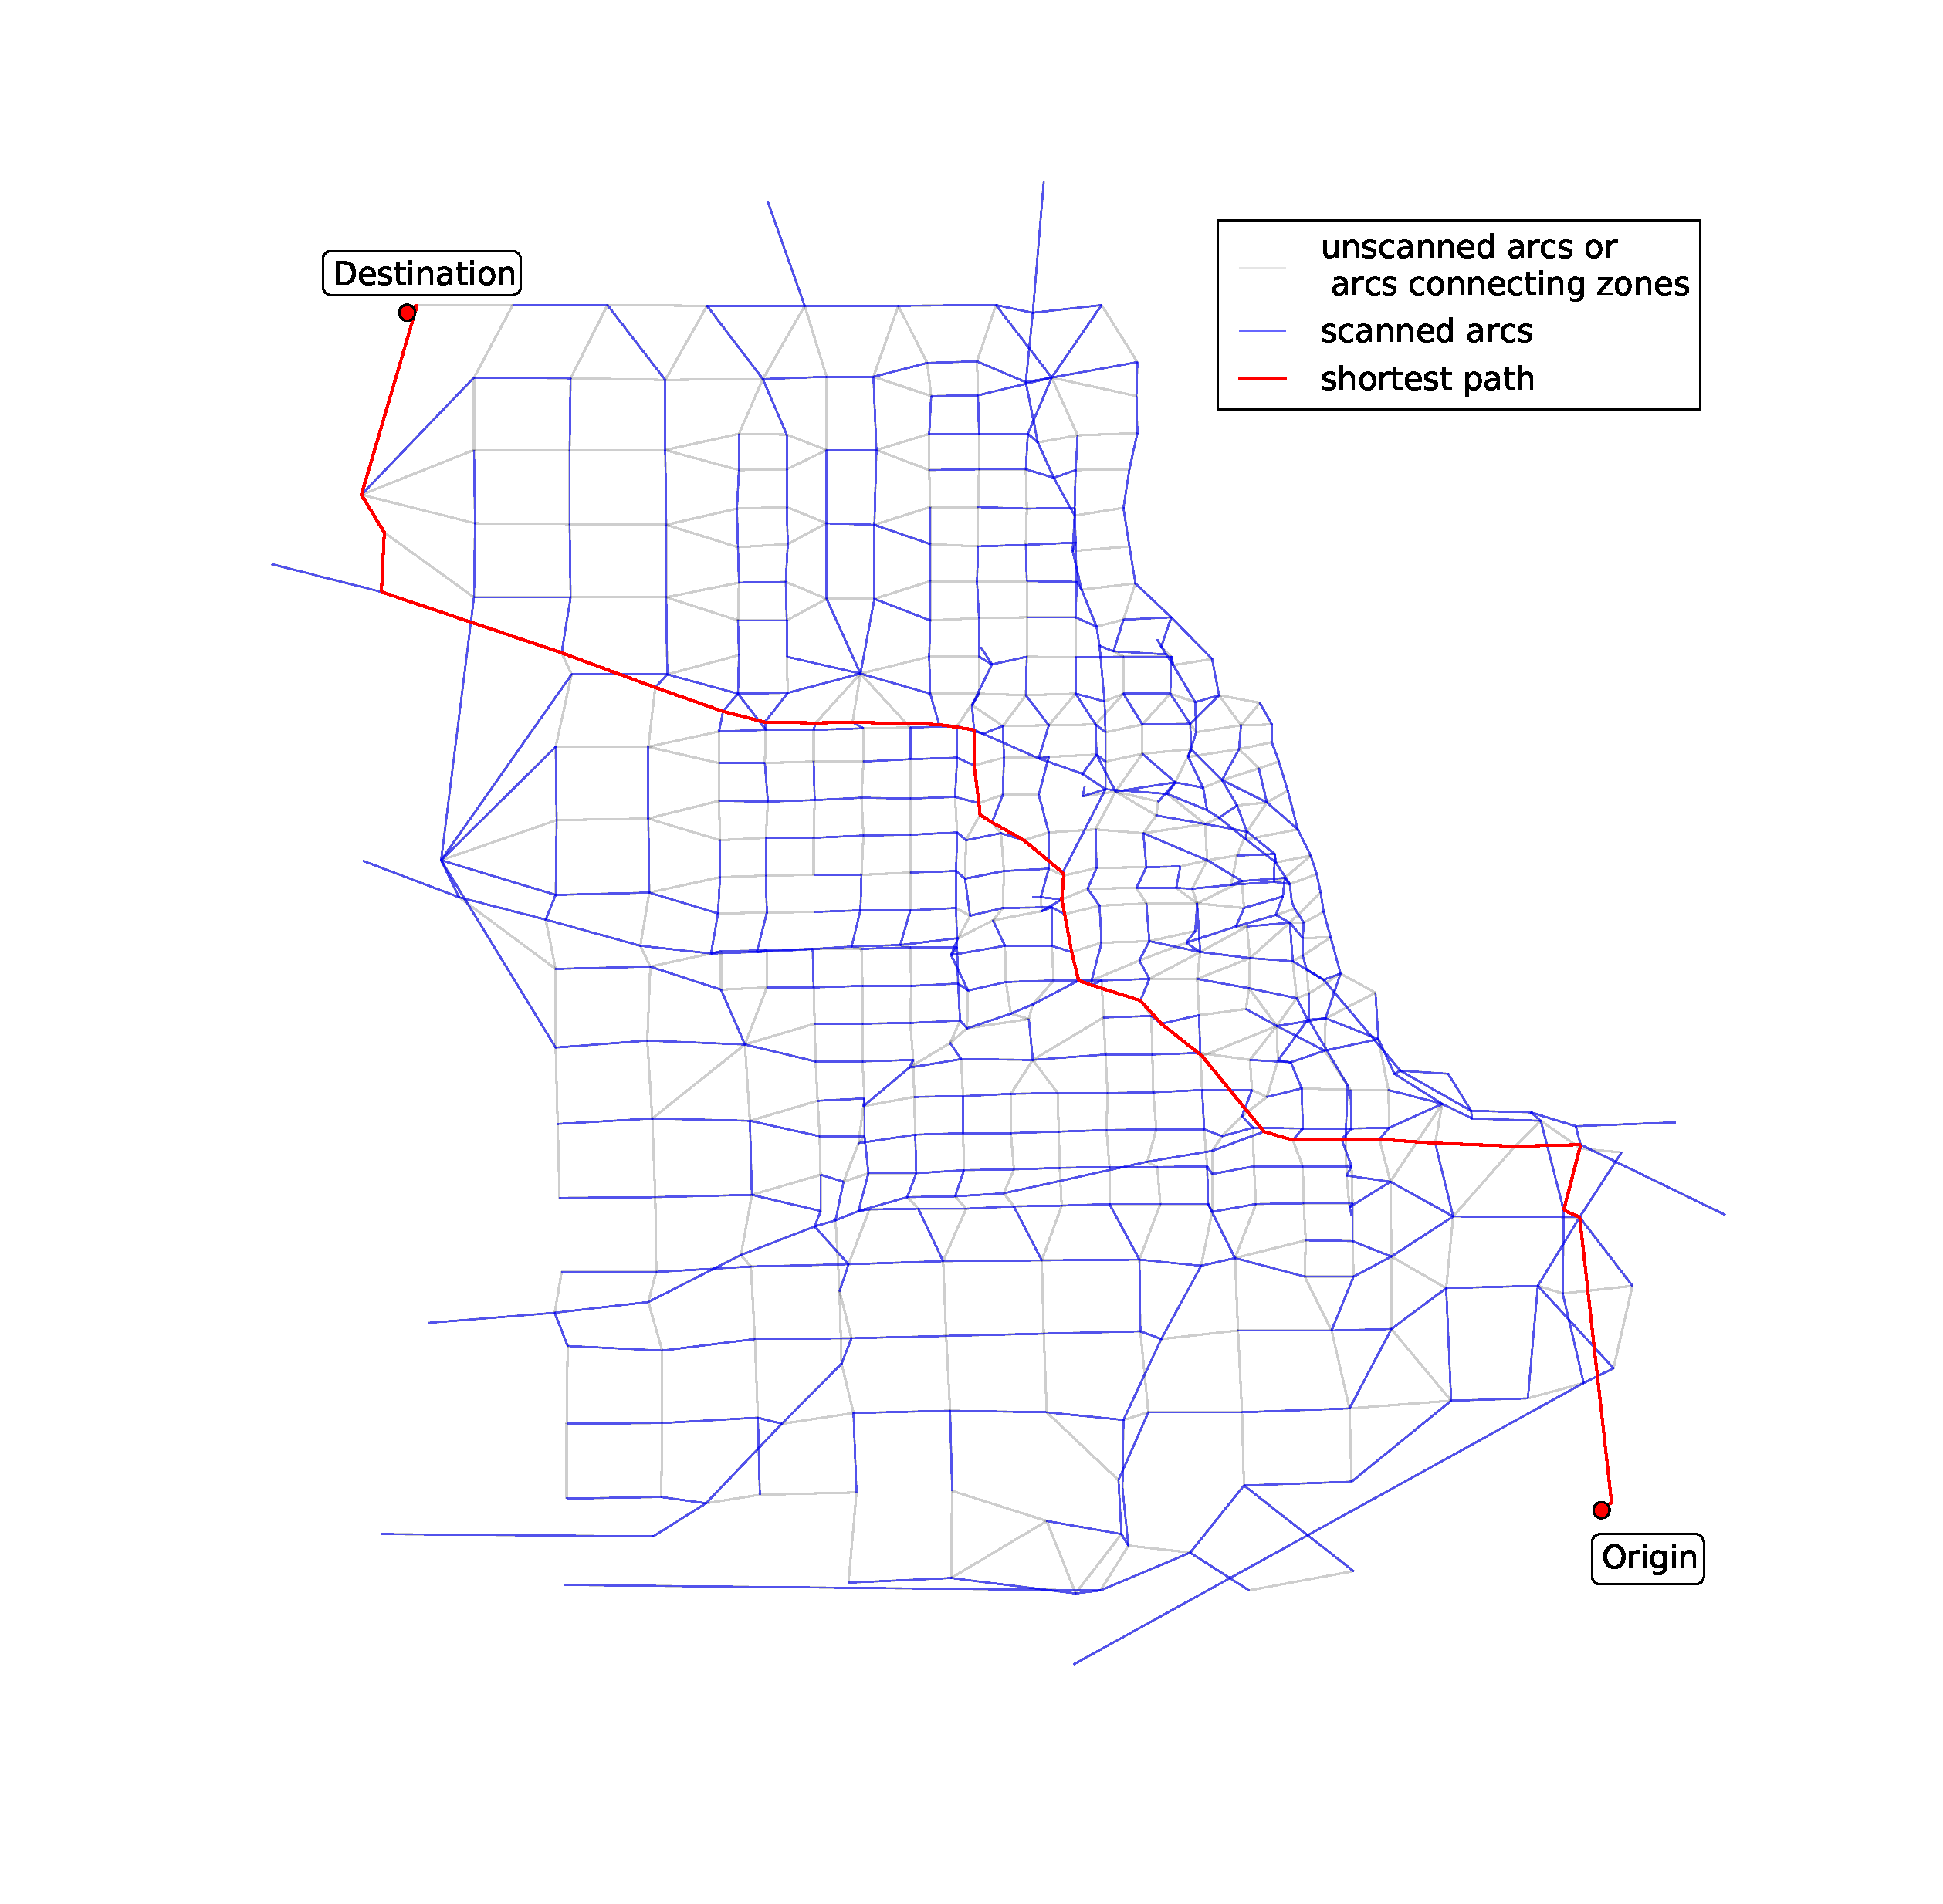
\includegraphics[width=\textwidth,trim=120px 120px 48px 120px,clip]{img/chicago_dijkstra}
        \caption{Dijkstra}
        \label{fig:chicago_dijkstra}
    \end{subfigure}%
    \begin{subfigure}{.5\textwidth}
        \centering
        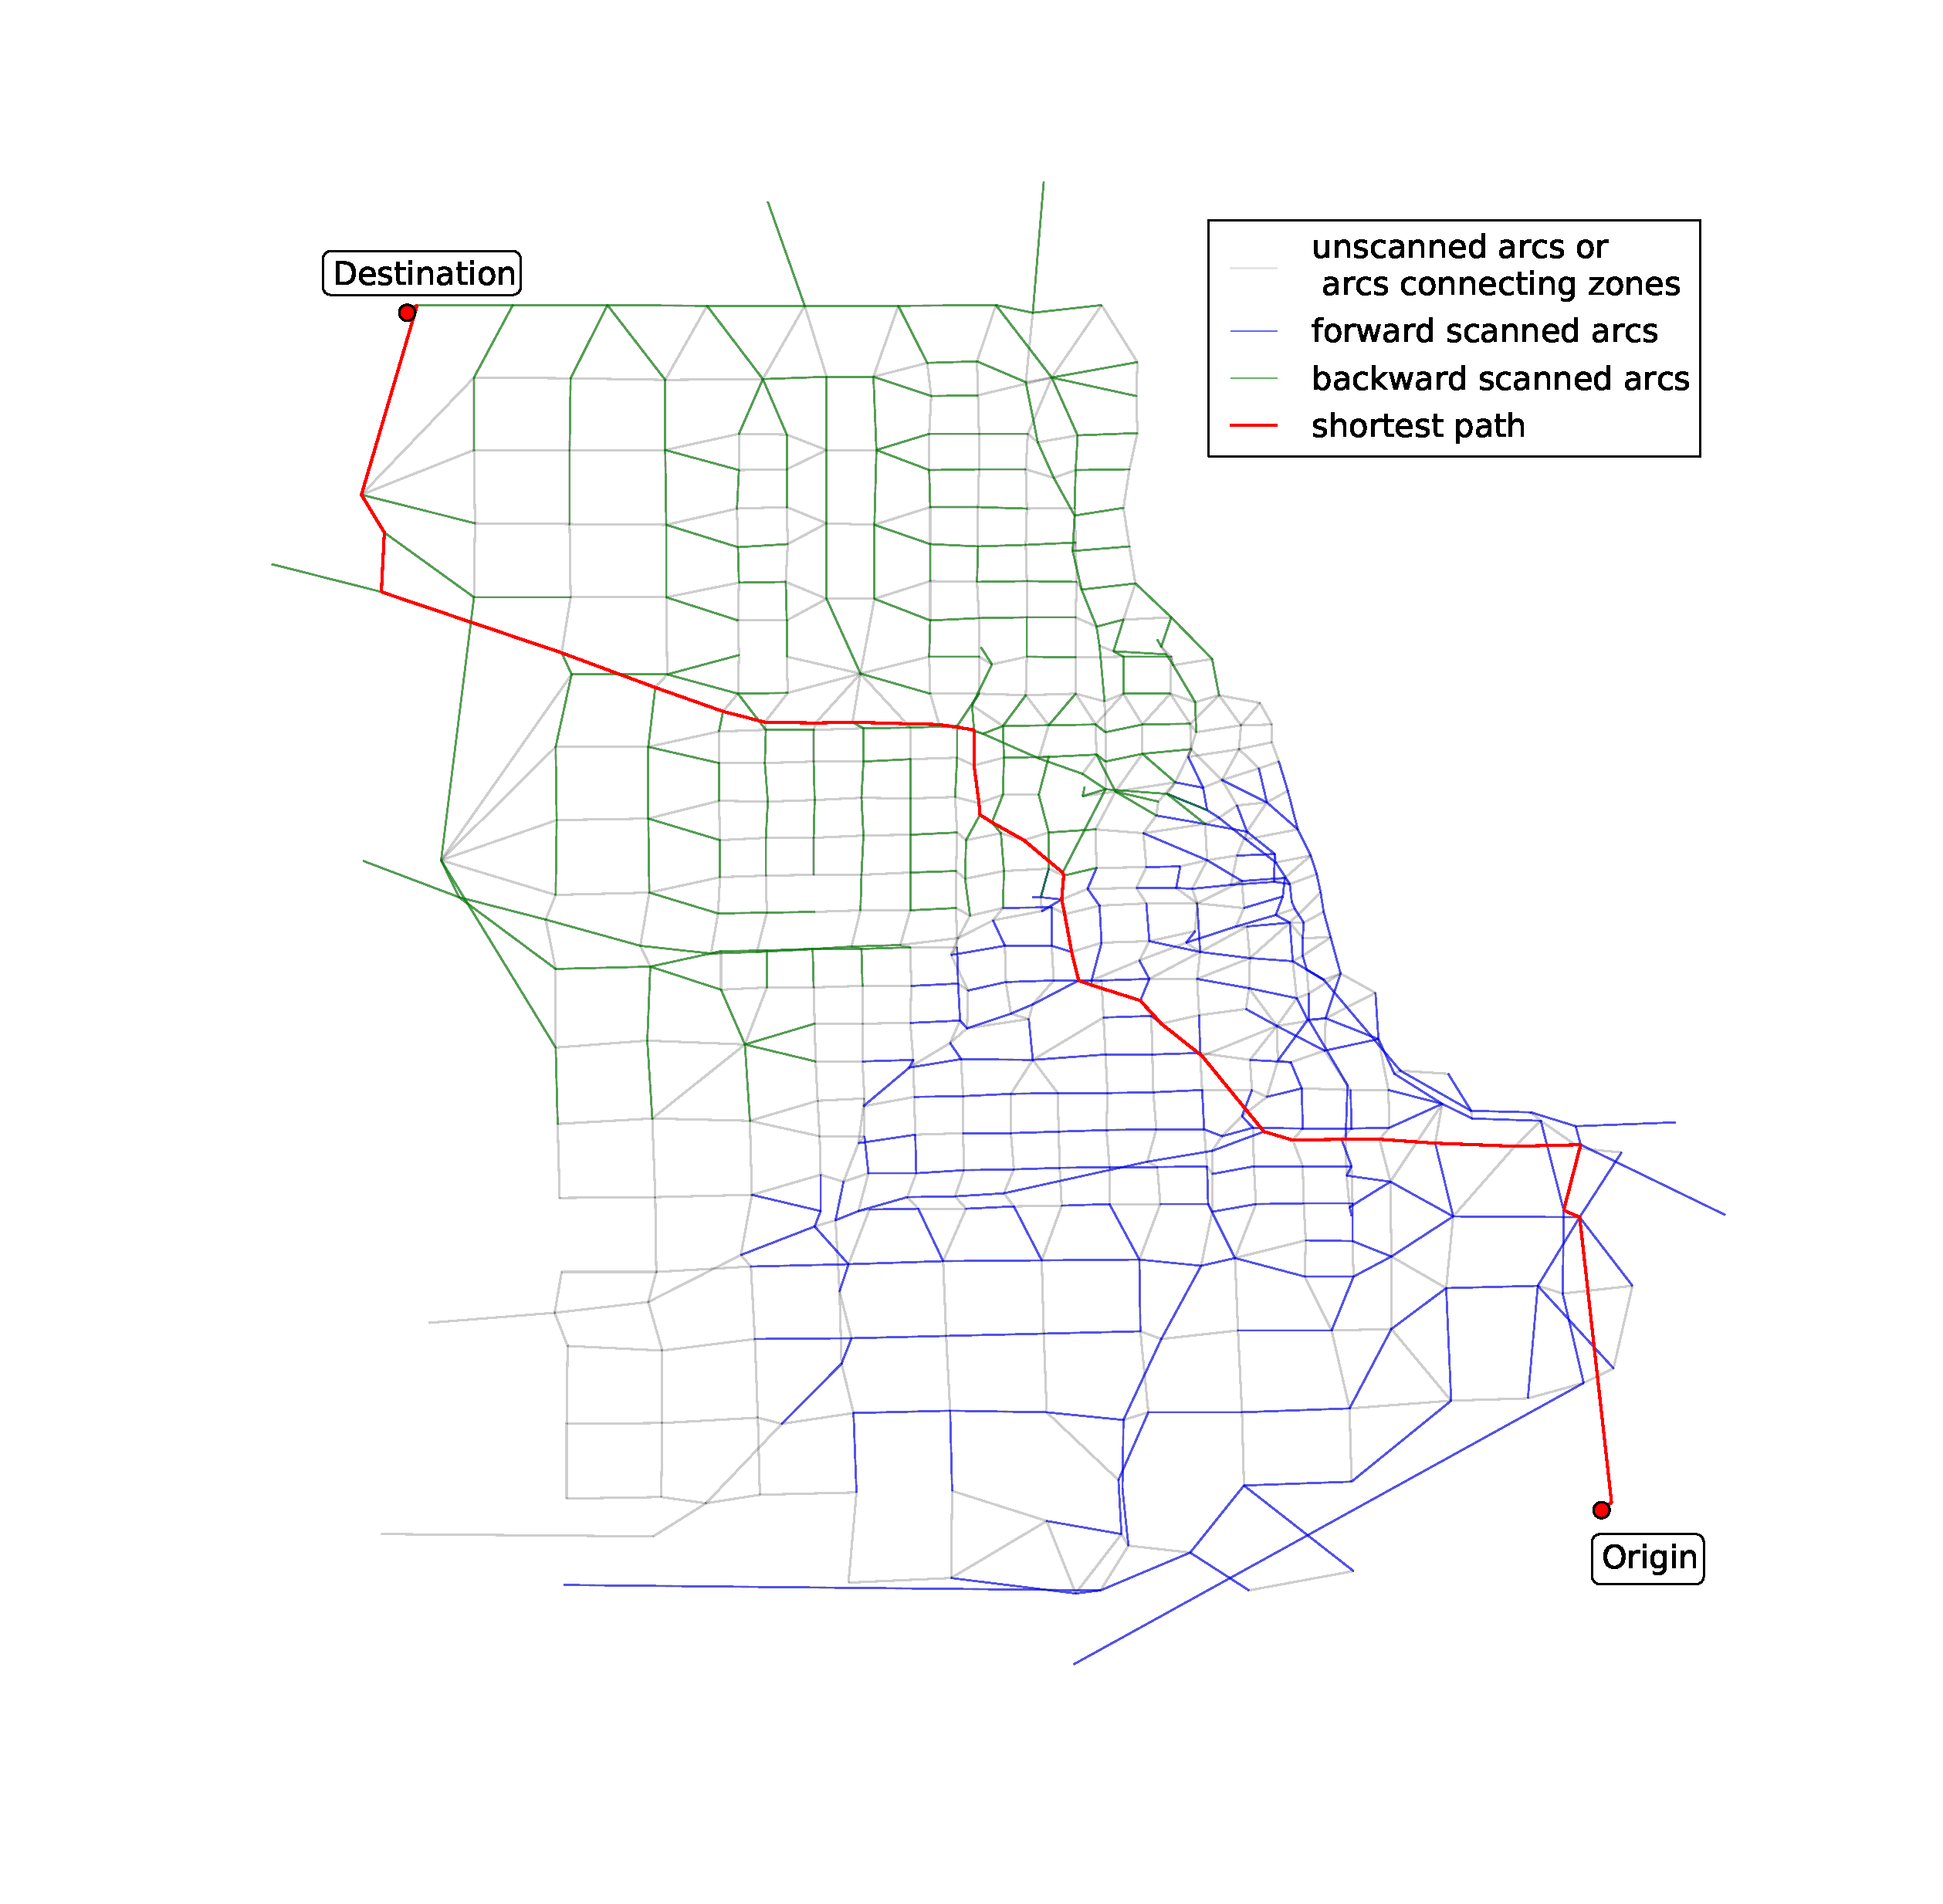
\includegraphics[width=\textwidth,trim=120px 120px 48px 120px,clip]{img/chicago_bidirect}
        \caption{Bidirectional Dijkstra}
        \label{fig:chicago_bidirect}
    \end{subfigure}
    \begin{subfigure}{.5\textwidth}
        \centering
        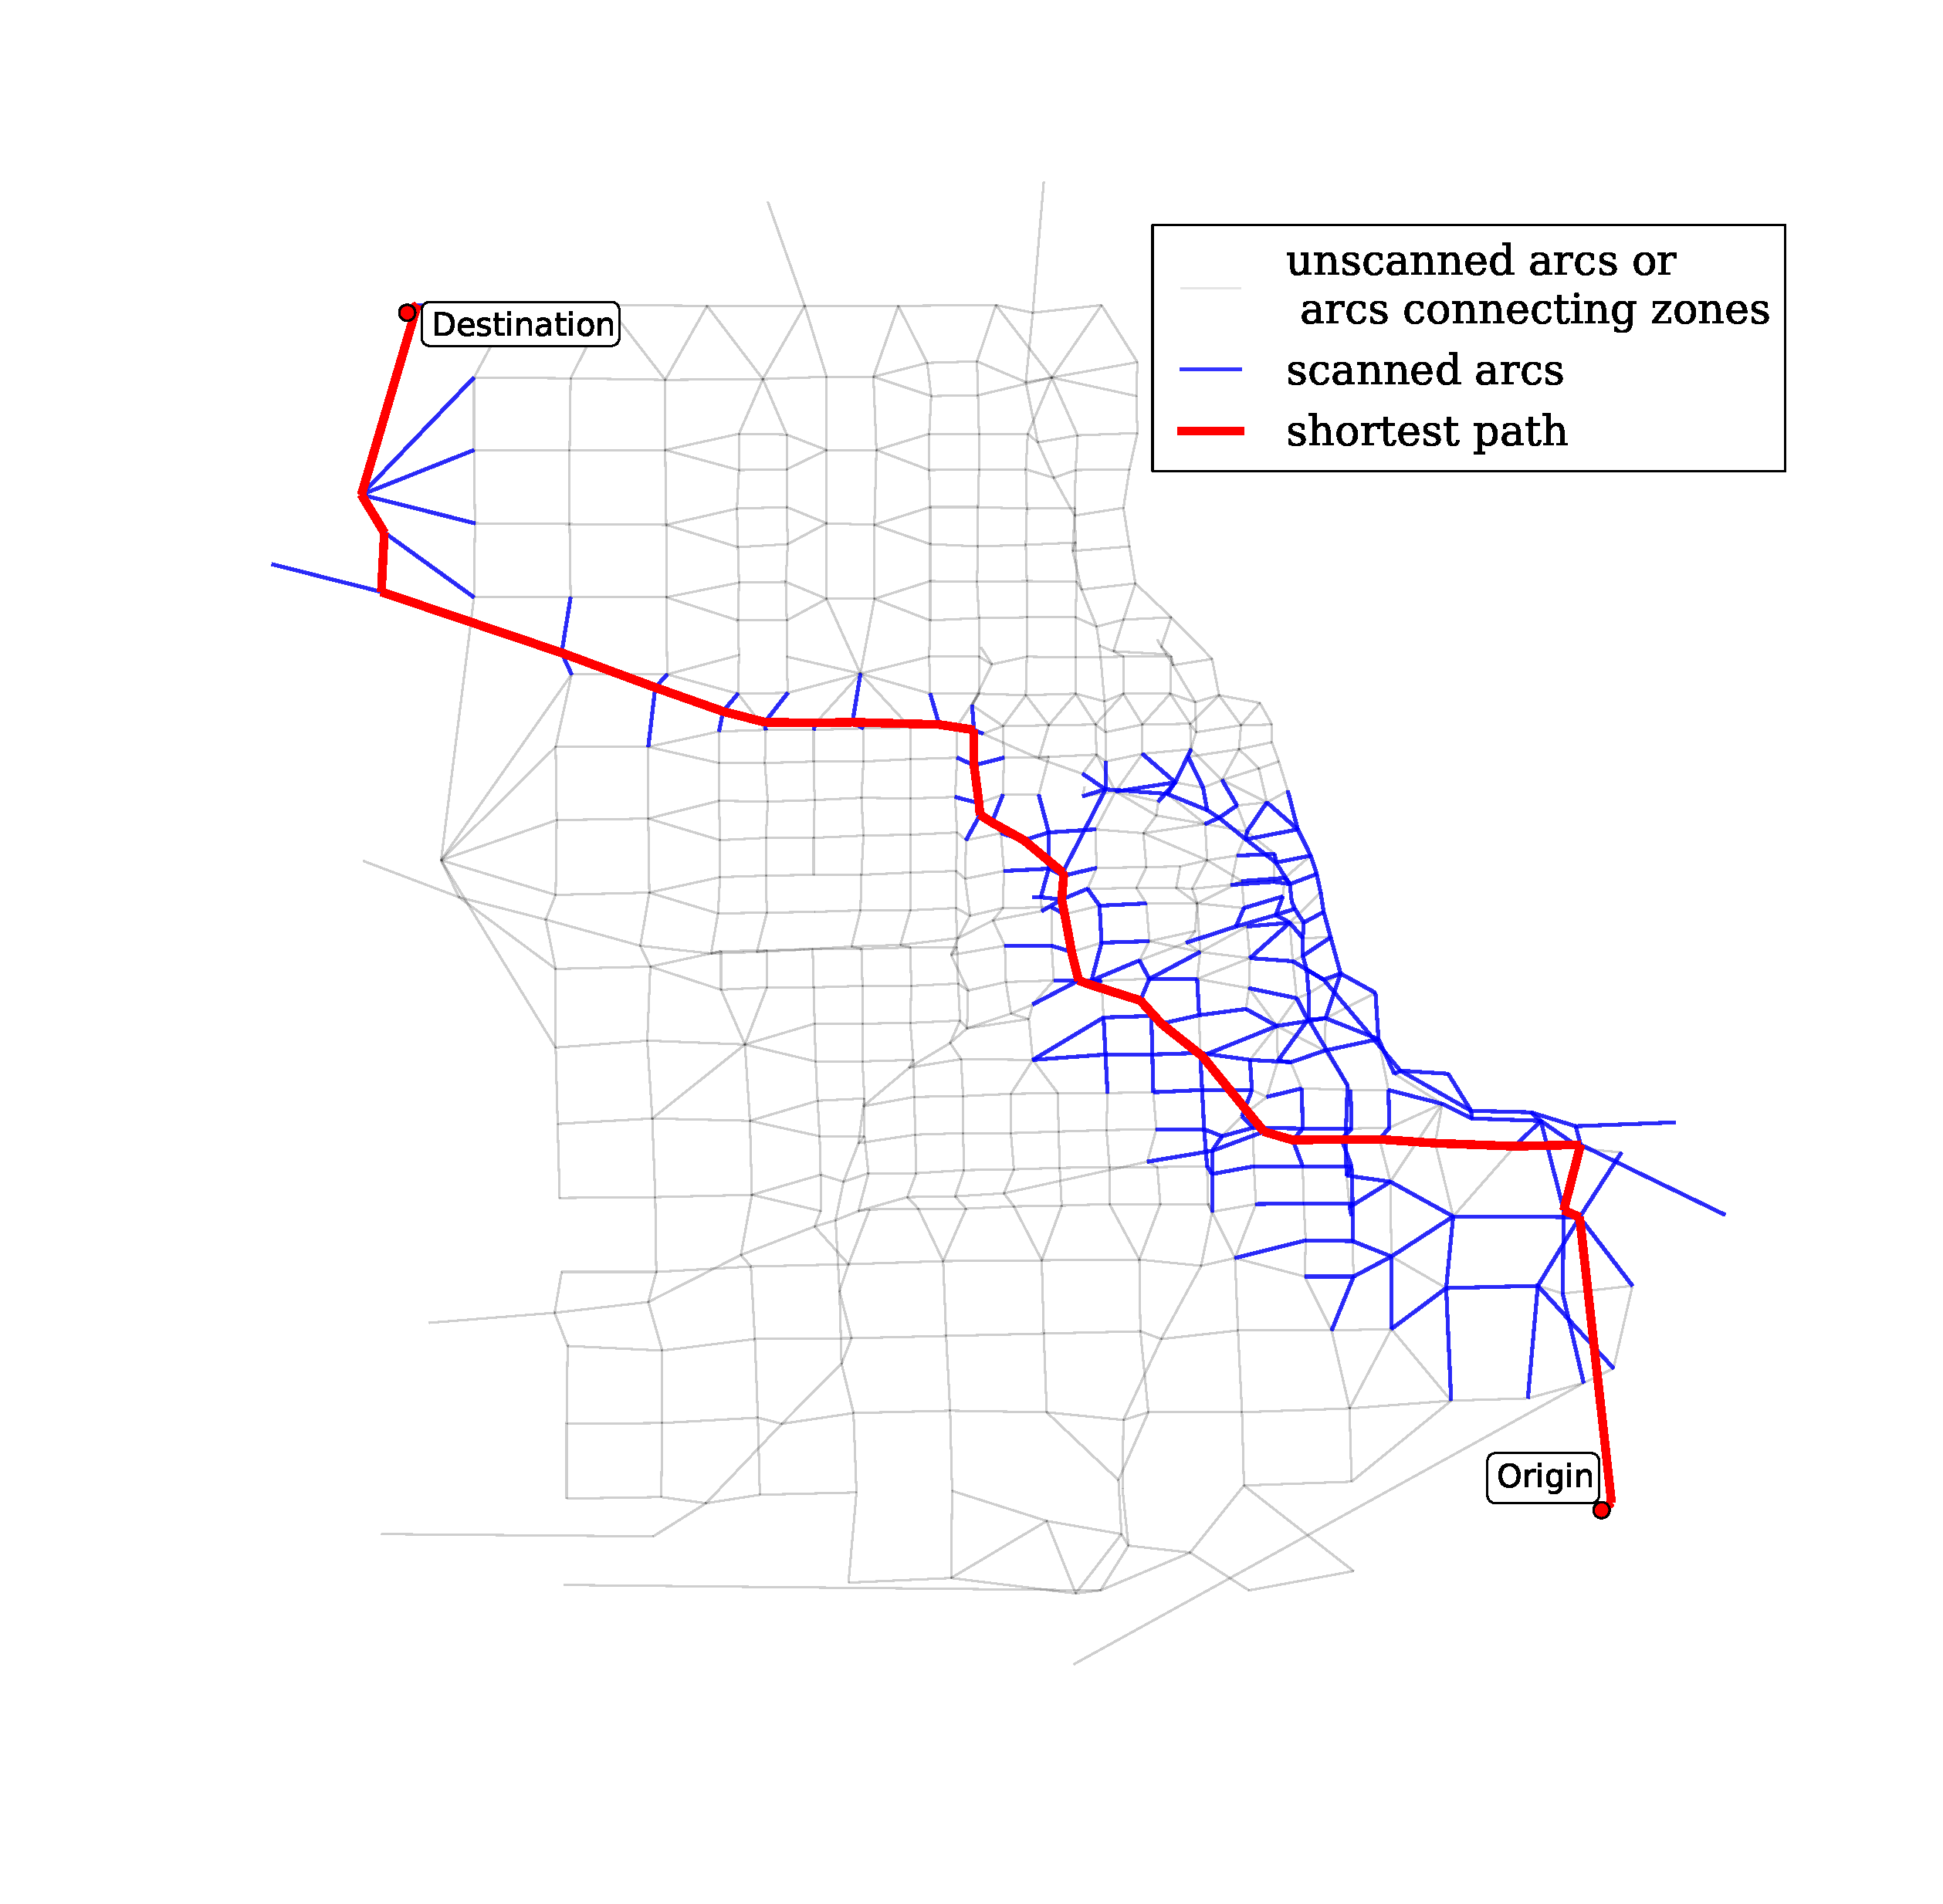
\includegraphics[width=\textwidth,trim=120px 120px 48px 0px,clip]{img/chicago_astar}
        \caption{A* Search}
        \label{fig:chicago_astar}
    \end{subfigure}%
    \begin{subfigure}{.5\textwidth}
        \centering
        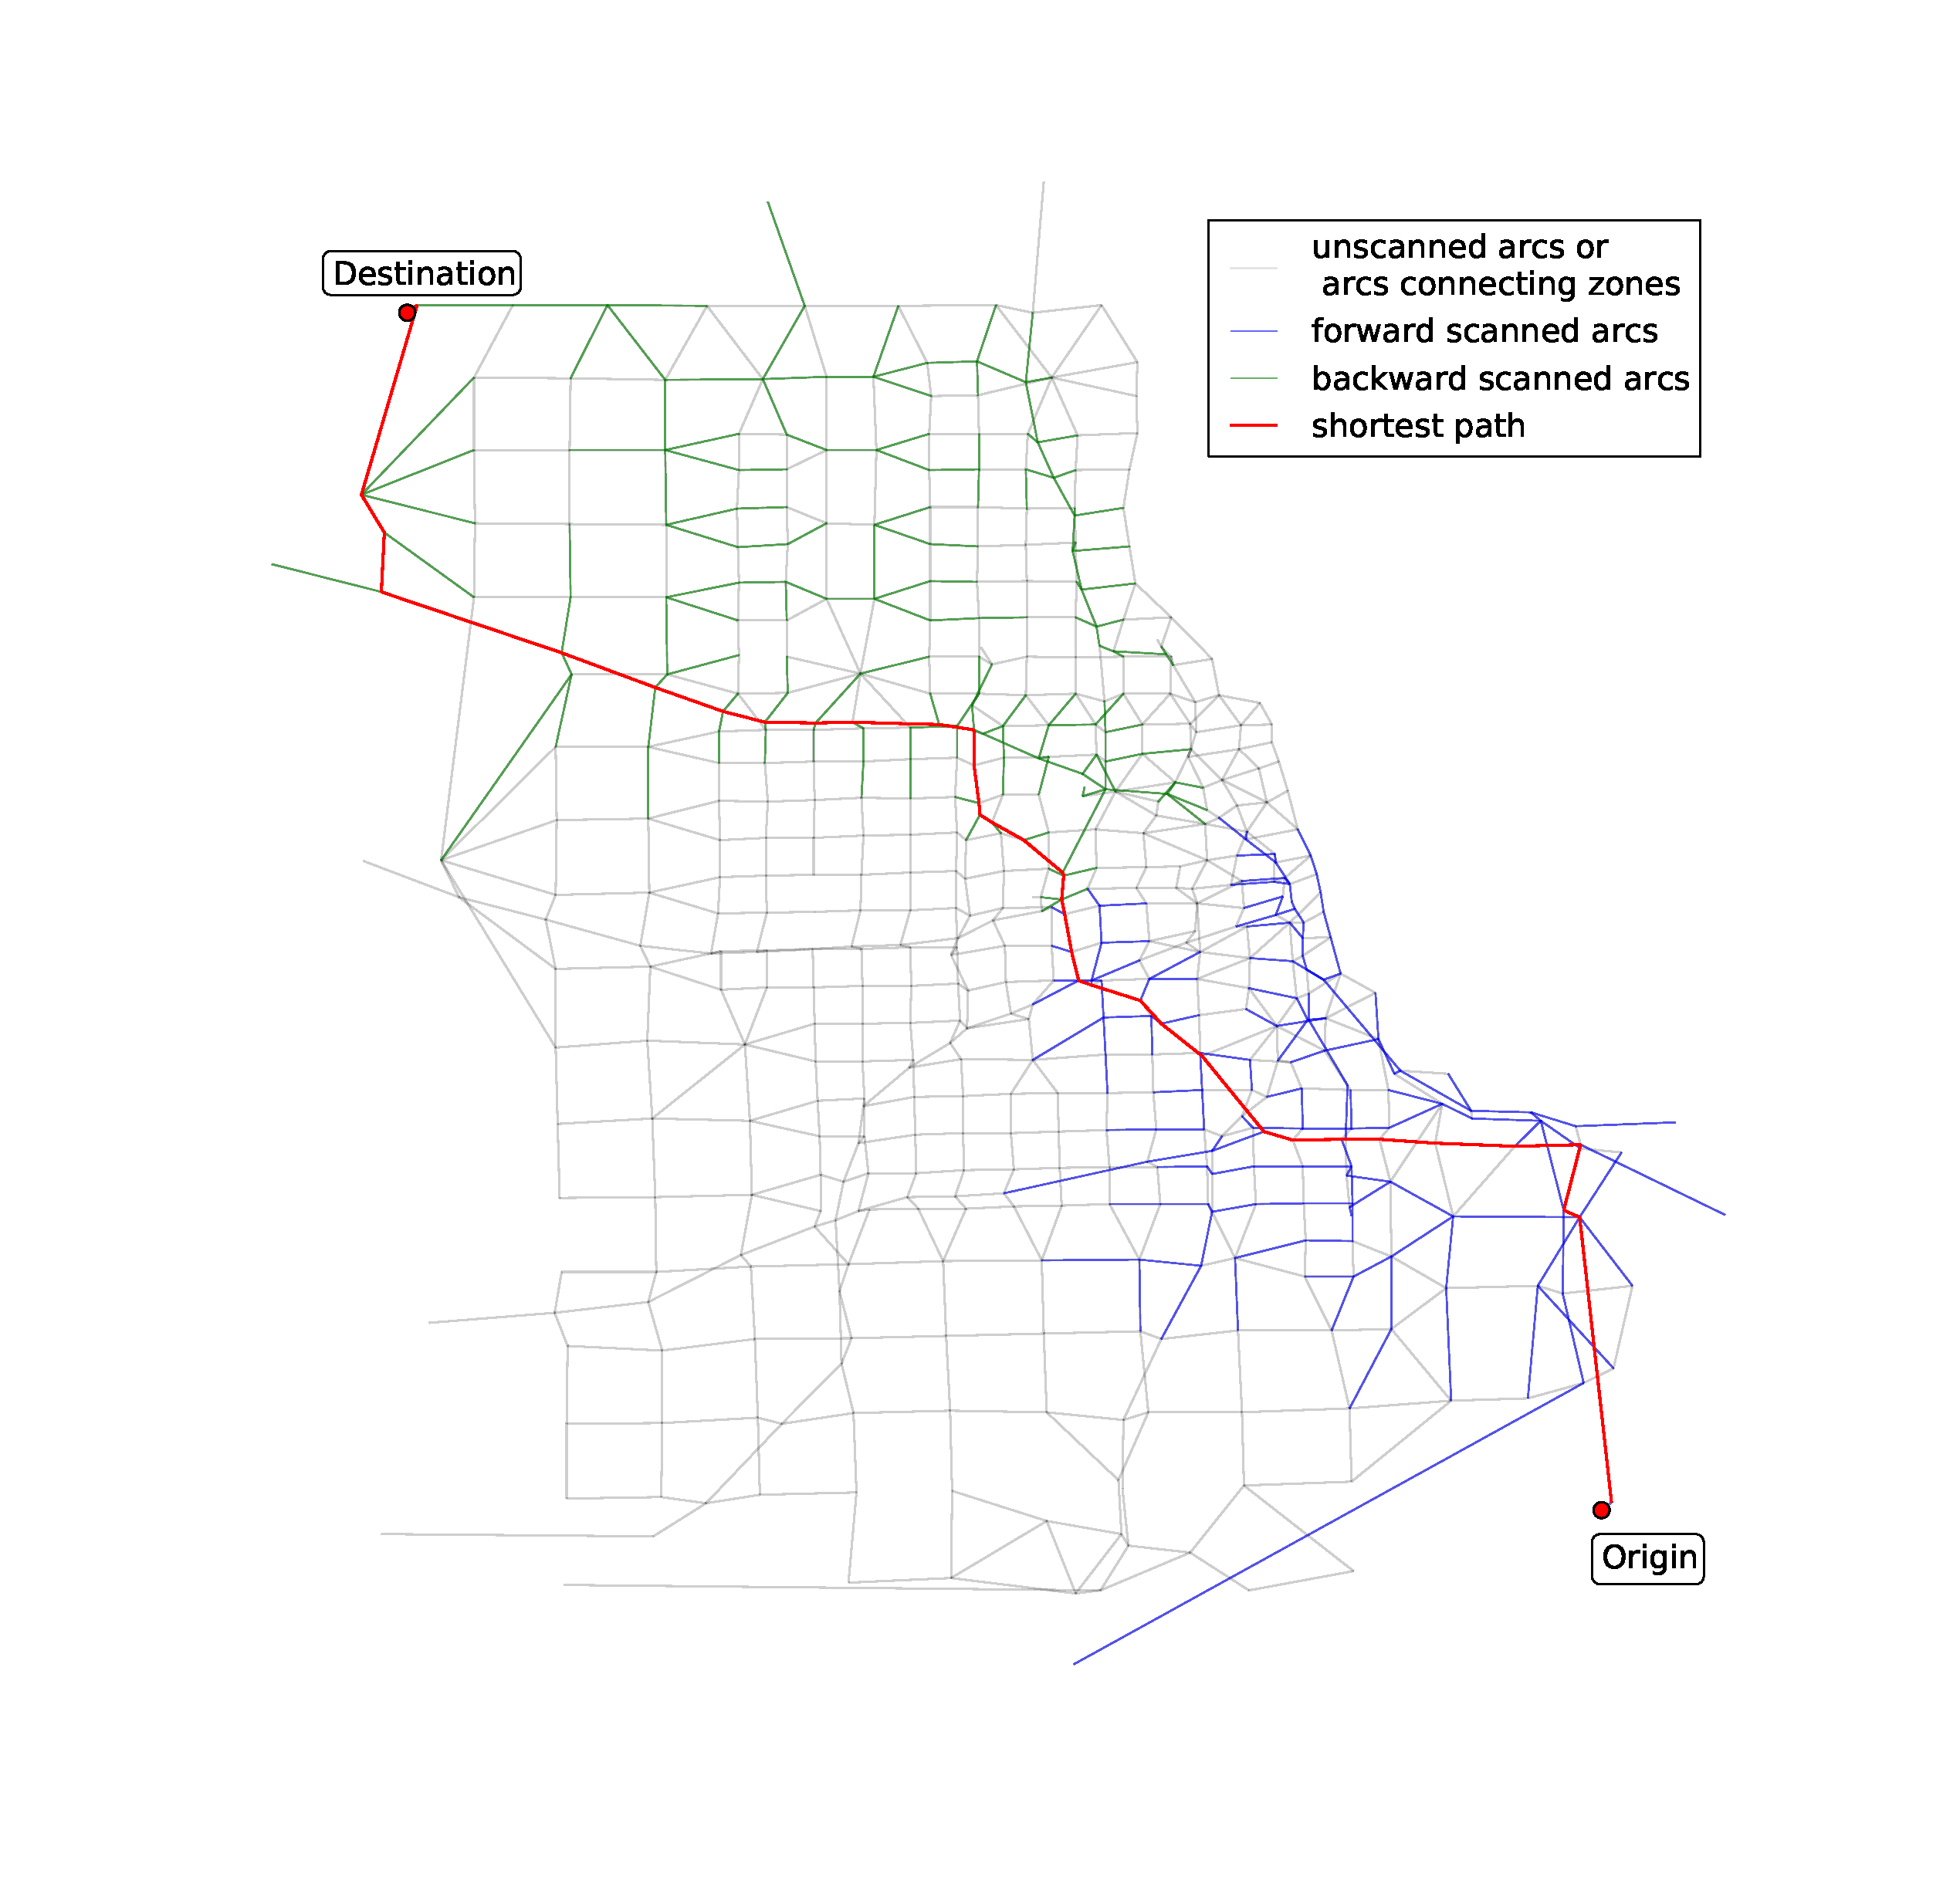
\includegraphics[width=\textwidth,trim=120px 120px 48px 0px,clip]{img/chicago_astar_bidirect}
        \caption{Bidirectional A* Search}
        \label{fig:chicago_astar_bidirect}
    \end{subfigure}
    \vspace{1em}
    \caption{Shortest path tree between two distant nodes in the ChicagoSketch Network}
    \label{fig:long_sptree}
\end{figure}

\begin{figure}
    \centering
    \begin{subfigure}{.5\textwidth}
        \centering
        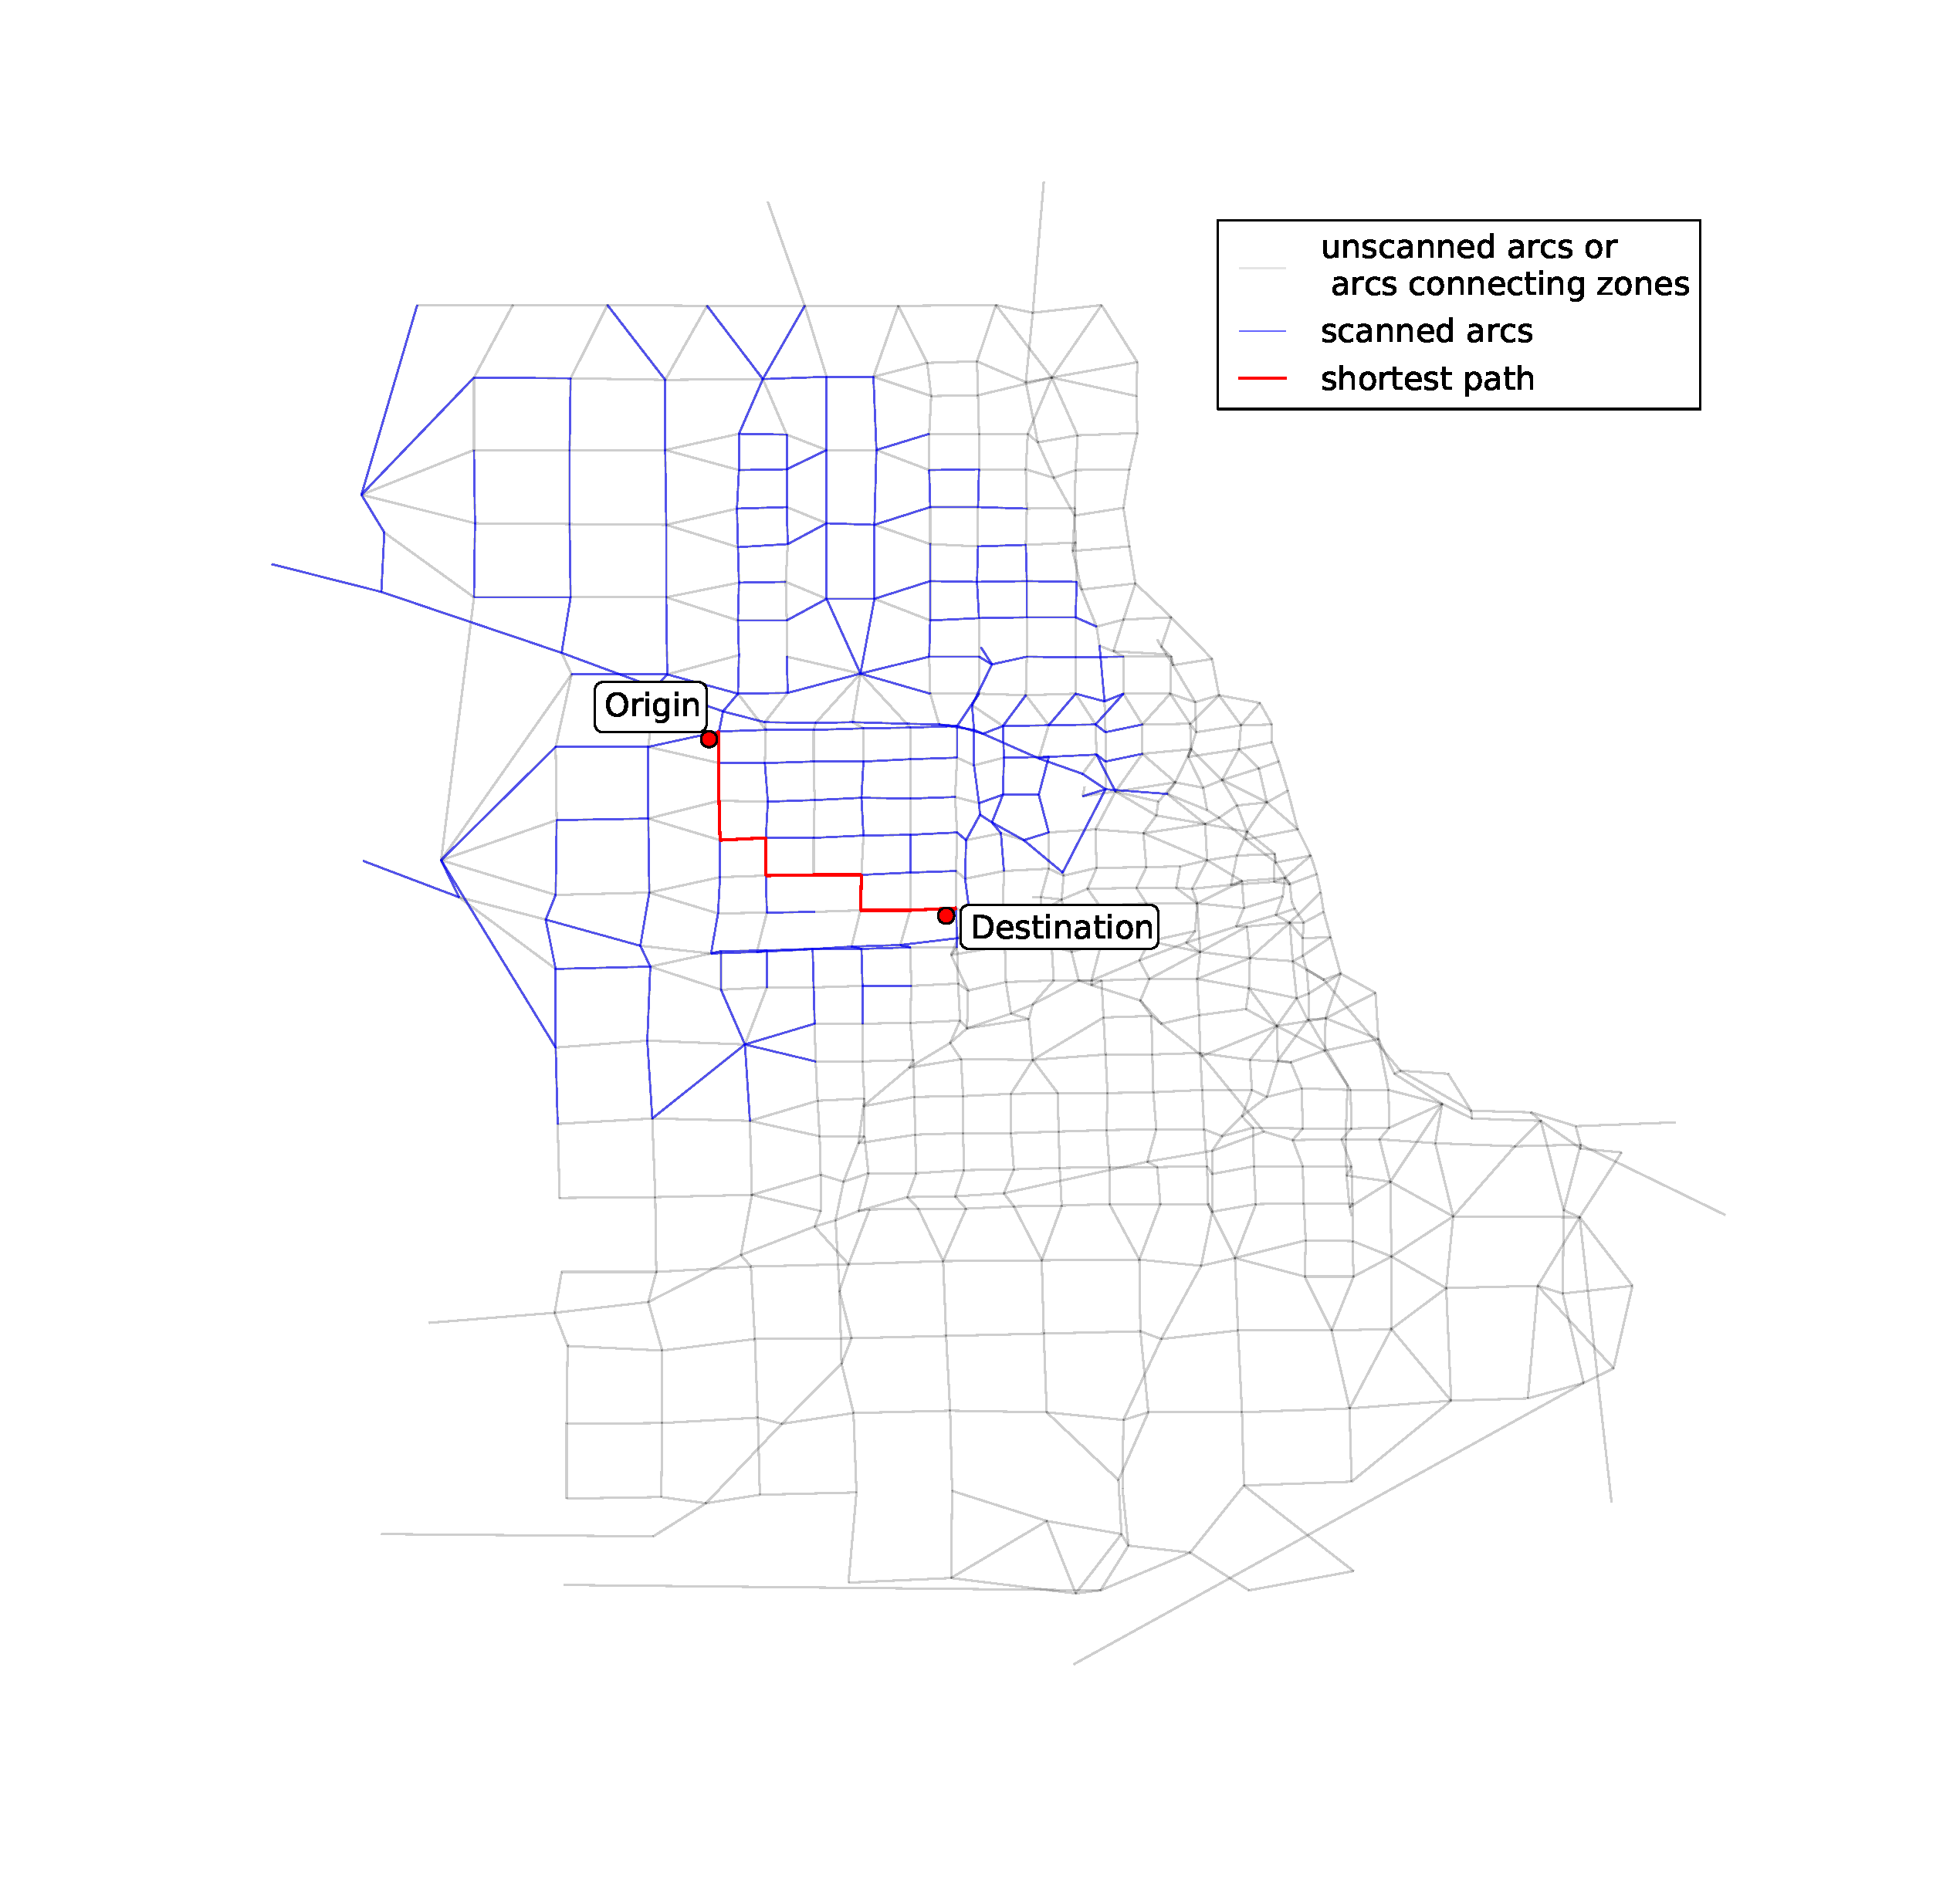
\includegraphics[width=\textwidth,trim=120px 120px 48px 120px,clip]{img/chicago_dijkstra2}
        \caption{Dijkstra}
        \label{fig:chicago_dijkstra2}
    \end{subfigure}%
    \begin{subfigure}{.5\textwidth}
        \centering
        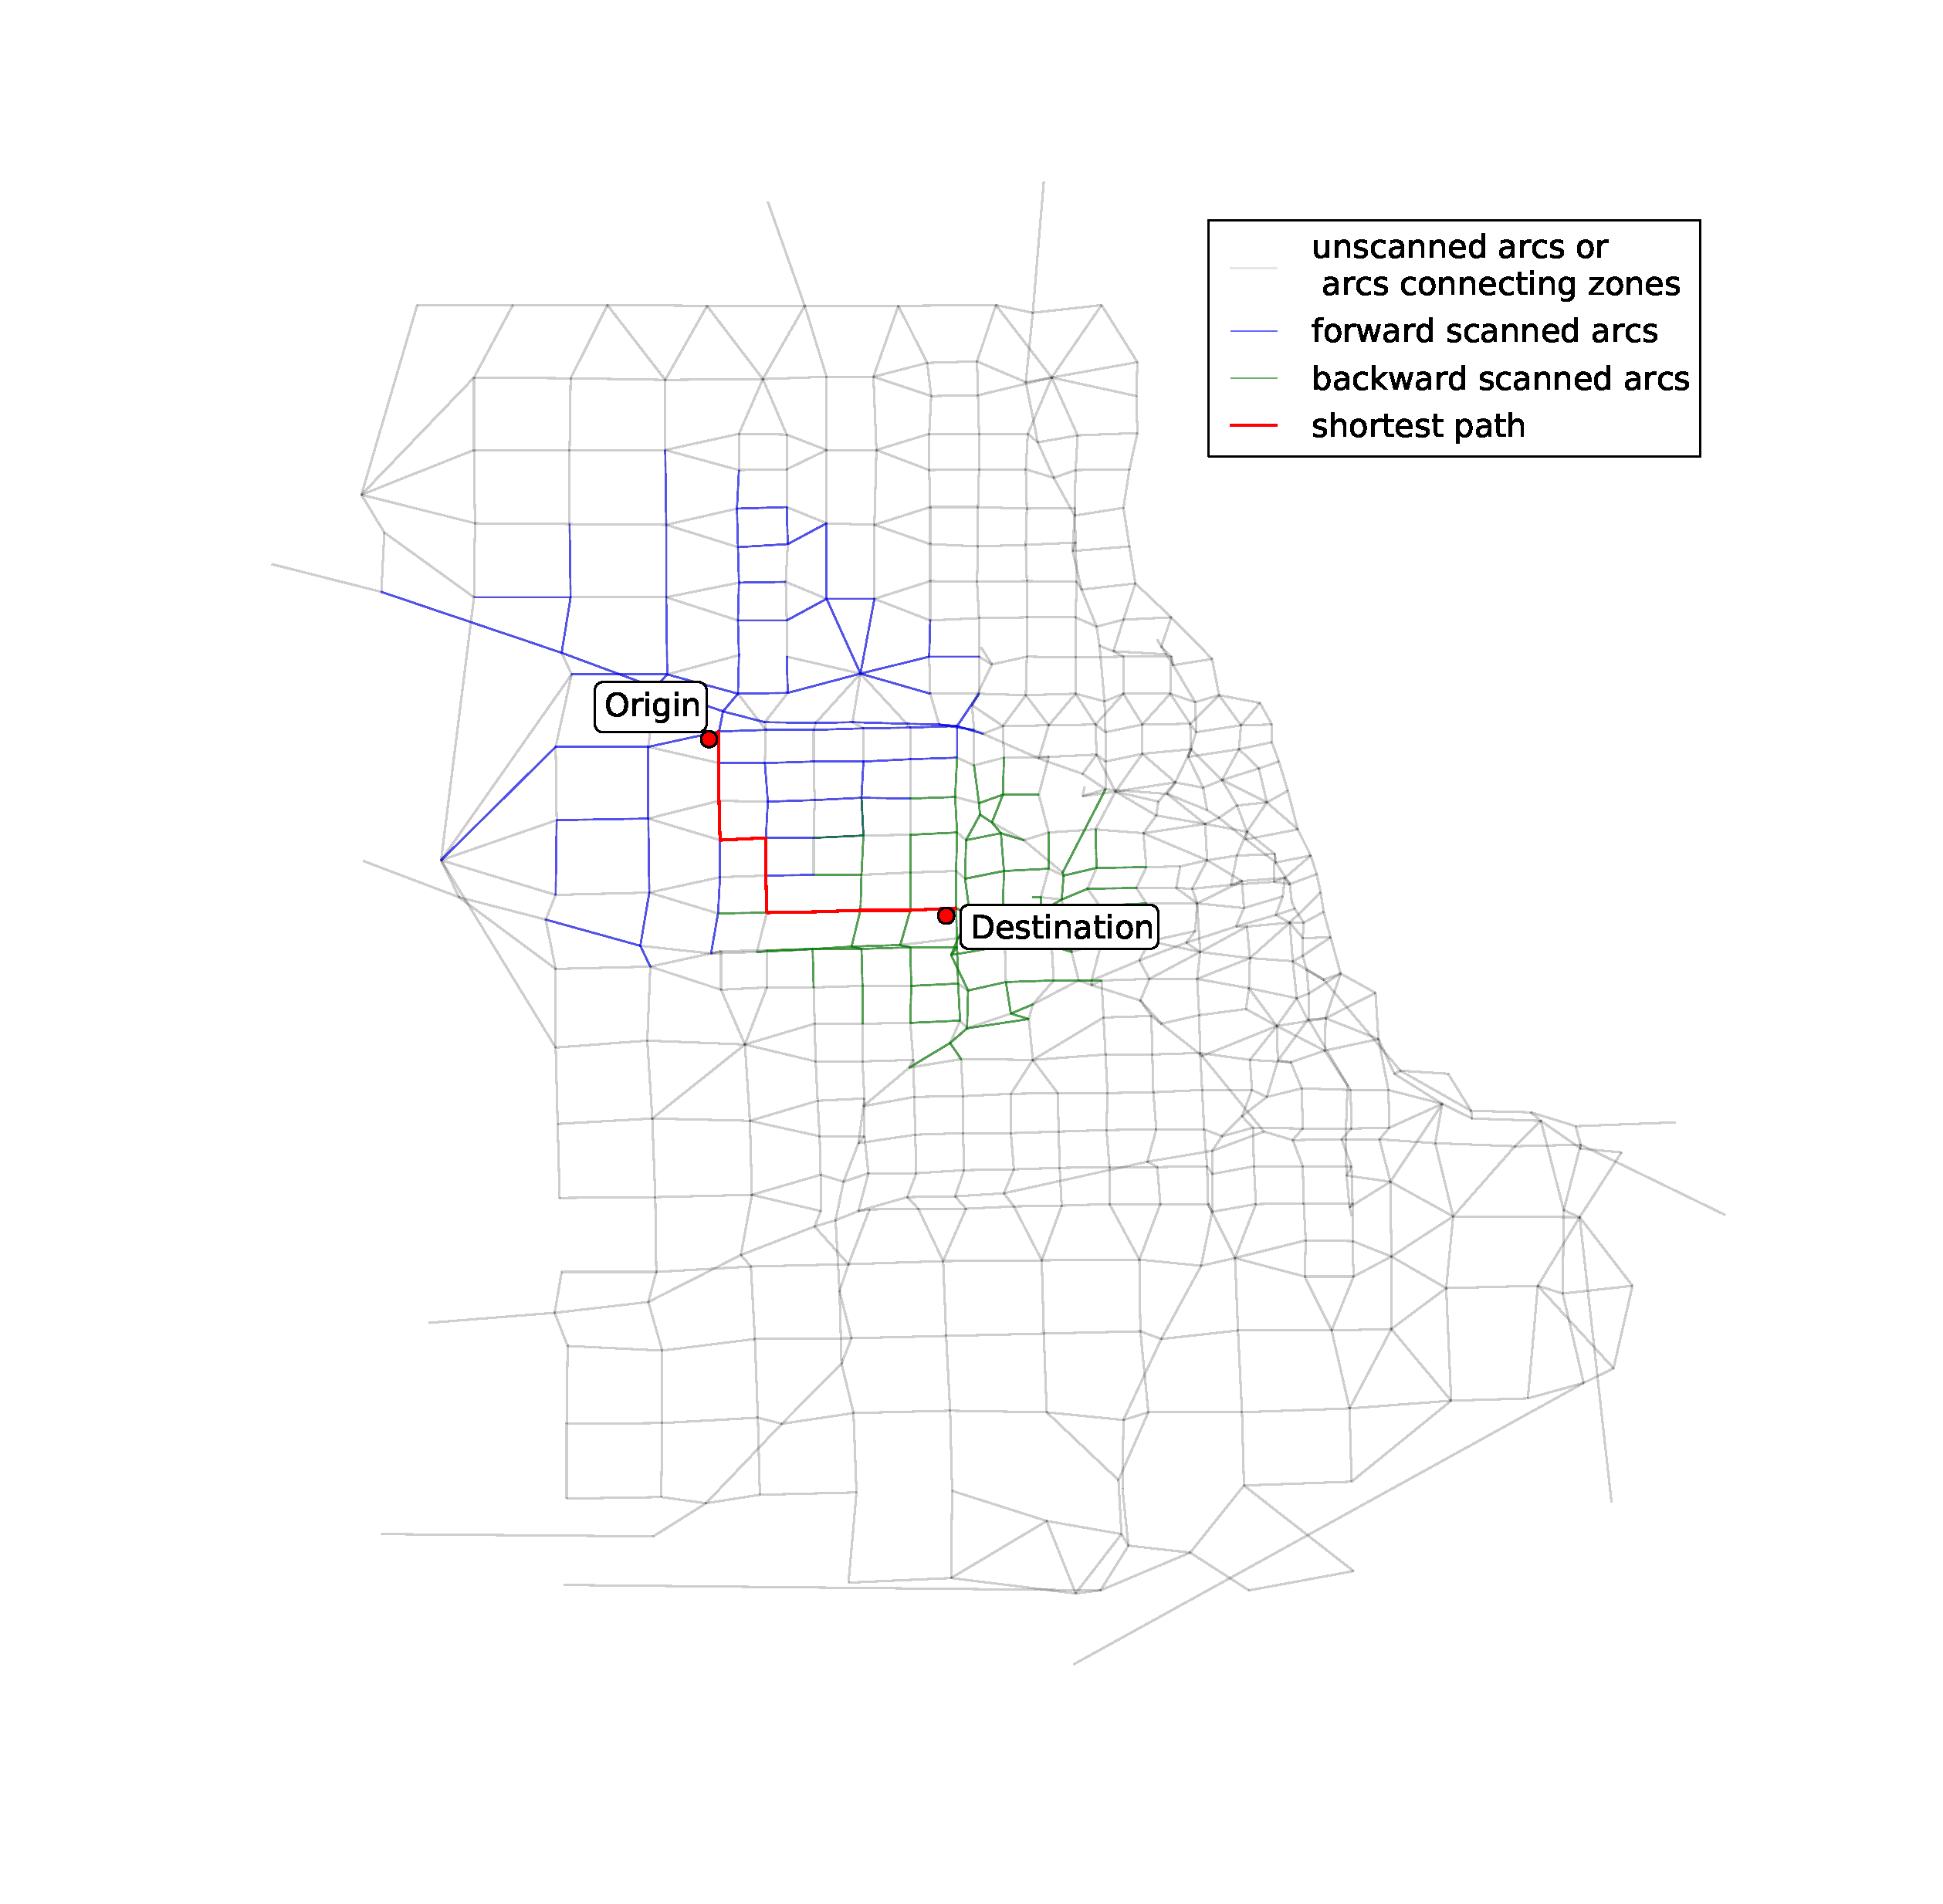
\includegraphics[width=\textwidth,trim=120px 120px 48px 120px,clip]{img/chicago_bidirect2}
        \caption{Bidirectional Dijkstra}
        \label{fig:chicago_bidirect2}
    \end{subfigure}
    \begin{subfigure}{.5\textwidth}
        \centering
        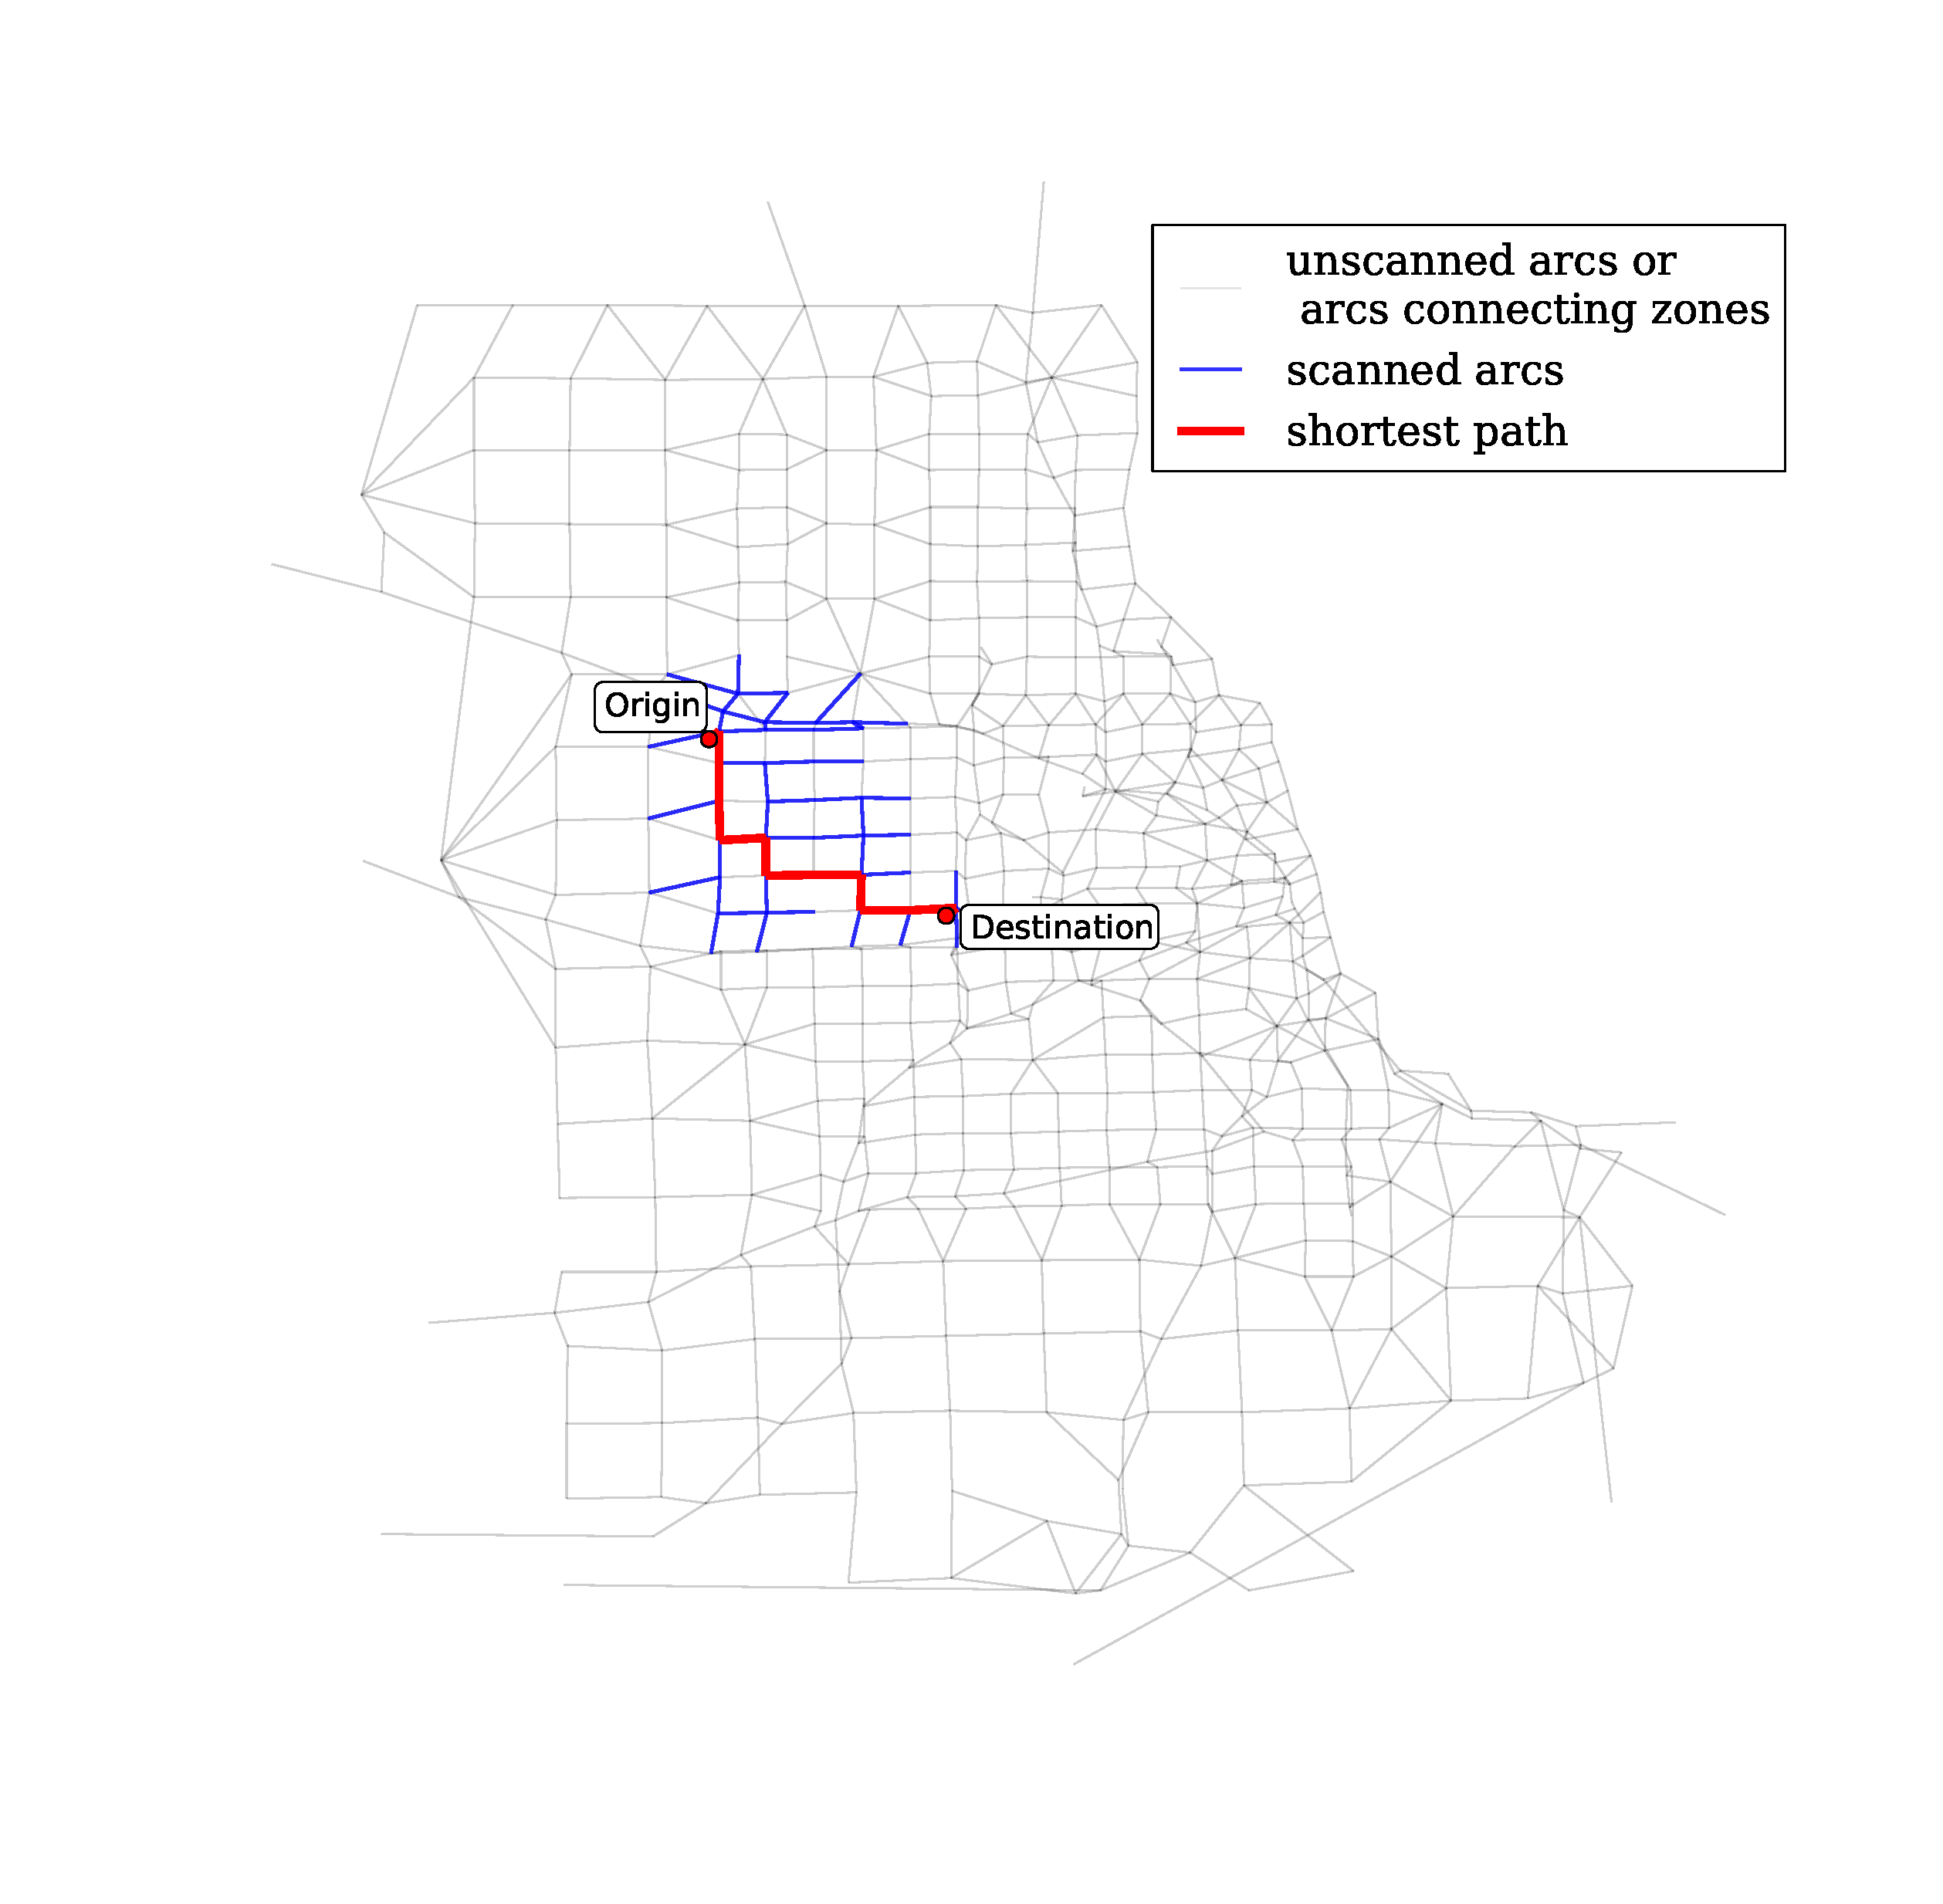
\includegraphics[width=\textwidth,trim=120px 120px 48px 0px,clip]{img/chicago_astar2}
        \caption{A* Search}
        \label{fig:chicago_astar2}
    \end{subfigure}%
    \begin{subfigure}{.5\textwidth}
        \centering
        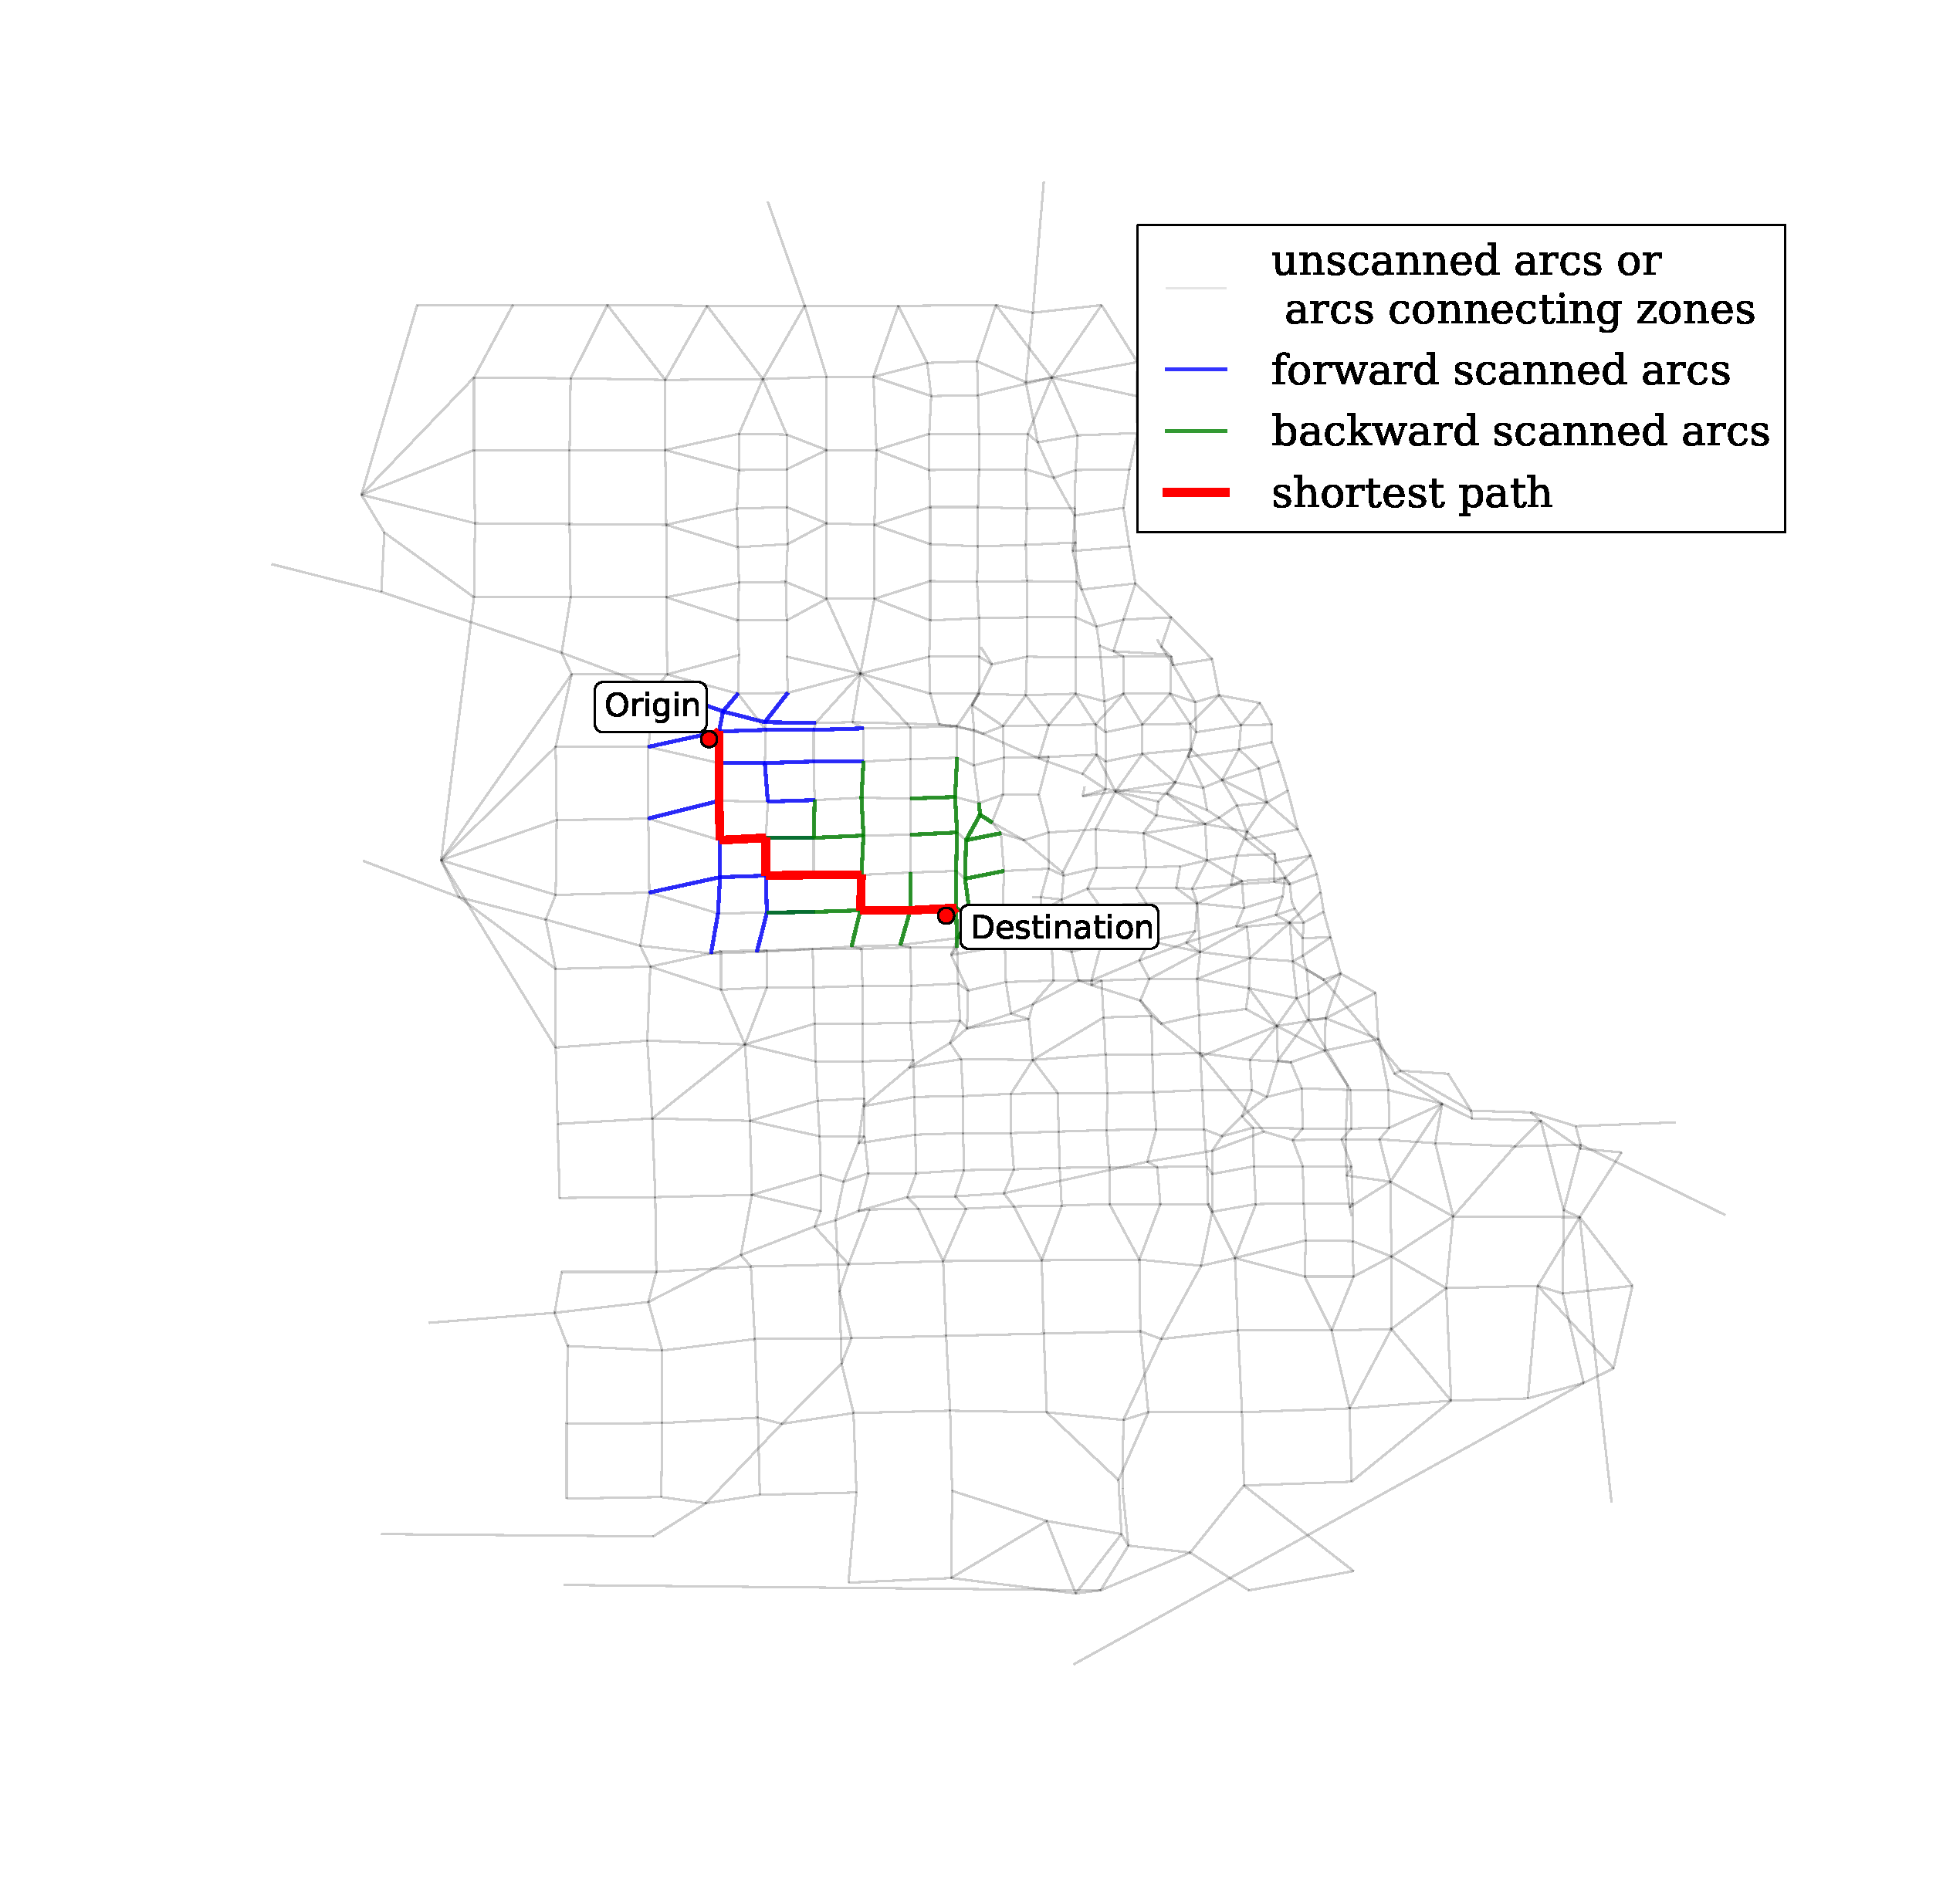
\includegraphics[width=\textwidth,trim=120px 120px 48px 0px,clip]{img/chicago_astar_bidirect2}
        \caption{Bidirectional A* Search}
        \label{fig:chicago_astar_bidirect2}
    \end{subfigure}
    \vspace{1em}
    \caption{Shortest path tree between two close nodes in the ChicagoSketch Network}
    \label{fig:short_sptree}
\end{figure}


\begin{comment}

All of these run times are slower than the STL version of the Heap.
Upon inspection,
it is found that the increase-key operation is used about between 5\% to 10\%
of the time,
\todo{not actual count yet}
which means the graphs are not dense enough for these Heap structures to outperform a
simple array based priority queue.
Comparing the Dijkstra and A* search algorithm's result,
we see an approximately 5 times improvement.
By looking at the shortest path tree generated
by the ChicagoSketch network,
there are only a few scanned nodes,
the path goes straight to the destination.
(TODO reference) says the closer the heuristic is to the actual distance,
the better/faster shortest path calculation,
by looking at the travel time function (Figure~\ref{fig:flowfunction}, we can see the slope
is really shallow near the start,
and by comparing the initial flow and final flow (TODO, data),
they are very close so the final flow is very close to the
initial flow,
which means the heuristic is a very good estimation,
which is our A* search is very fast.
\end{comment}


\section{Results on skipping shortest path calculations}
In this section we consider skipping shortest path calculations in the iterative Path Equilibration algorithm discussed in Section~\ref{section:avoid}.

First we investigate how the shortest paths change during a complete run of the Path Equilibration algorithm.
Figure~\ref{fig:sp_change} shows 
the percentage of how many times each O-D pairs' shortest path change during the 26 iterations of the algorithm run on the ChicagoSketch network.
It is shown that most of the shortest paths only change a few times during the complete run of the Path Equilibration algorithm.
This entails that after the first dozen of iterations,
the rest of the algorithm spends its time balancing only a few shortest paths.
From this observation,
we can develop a strategy of skipping some shortest path calculations
if they do not change in the previous two iterations.
This result is shown in Figure~\ref{fig:skip_n} for the Terrassa and ChicagoSketch network, 
where an arbitrary numbers of skipping are chosen.

The Terrassa network mentioned above is a small network with 55 zones, 1609 nodes, 3264 links and 2215 O-D pairs.
Using A* search,
the algorithm takes 415 iterations to converge due to its complicated supply and demand description.

Figure~\ref{fig:terrassa_skip_n} shows the A* search run time on Terrassa network.
The strategy is to skip the next 15, 25, 50, 100 and 200 calculations for the O-D pair that did not change its shortest path in previous two iterations.
This strategy worked very well as all of the run times are reduced by half,
with only some change in the total number of iterations.
Figure~\ref{fig:chicago_skip_n} shows the same information on the ChicagoSketch network, with skipping the next 5, 10 15 and 20 iterations.
There are only a slight reduce of run times,
with a relatively large increase in the total number of iterations.
The strategy did not work well due to its large network size.

The problem with this strategy is that we have to know how many iterations the algorithm will take and choose an appropriate number that is less than that,
this is because choosing a `bad' skipping number will result either unnecessary computations or have no effect on reducing the run time.

The next strategy we explore is to skip the next shortest path calculation randomly.
The advantage of this strategy is that it does not need the number of iterations it will compute,
but the disadvantage is that the run time may vary between different runs.
Figure~\ref{fig:terrassa_random_n} shows the A* search run time on the Terrassa network with skipping the current O-D pair shortest path calculation using probabilities of 0.3, 0.4, 0.5, 0.6 and 0.7.
In this case the run time dropped quite significantly for 0.5 probability,
while the other probabilities all have reduced the run time by some amount.
Figure~\ref{fig:chicago_random_n} shows the same strategy on the ChicagoSketch network.
Again this time there is no significant reduction in run time but all of the run times are reduced slightly.

Since the skipping shortest path strategy seems to work well,
and because only small networks have been experimented so far,
we will now experiment this strategy along with A* search on two more huge networks.

The networks that is going to be experimented are the Philadelphia and ChicagoRegional network. 
The Philadelphia network consists of $1,525$ zones, $13,389$ nodes, $40,004$ links and $1,149,795$ O-D pairs.
The ChicagoRegional network consists of $1,790$ zones, $12,982$ nodes, $39,018$ links and $2,296,227$ O-D pairs.
It is interesting to note that these two networks consist of 1 and 2 millions of O-D pairs, which means they require 1 and 2 millions shortest path calculations just for 1 iteration of the Path Equilibration algorithm.
The run time comparisons are shown in Table~\ref{table:runtime_large_network}.

Table~\ref{table:runtime_large_network} show both the A* search and A* with 0.5 probabilities of randomly skipping an shortest path calculation on the two networks mentioned above.
The random skipping strategy has approximately 25\% and 27\% run time improvement on the Philadelphia and ChicagoRegional respectively.

\begin{table}[H]
    \begin{tabular}{p{0.3\textwidth} | c c}
        & Philadelphia & ChicagoRegional \\ \cmidrule(lr){2-2} \cmidrule(lr){3-3}
        A* search & 7.69 hours & 33.26 hours \\ 
        A* with 0.5 probability of randomly skipping & 5.75 hours & 24.18 hours\\
    \end{tabular}
    \caption{Run time of A* search and the randomly skipping strategy on Philadelphia and ChicagoRegional network}
    \label{table:runtime_large_network}
\end{table}


\todoin[inline]{maybe need random analysis}
\begin{figure}[H]
    \centering
    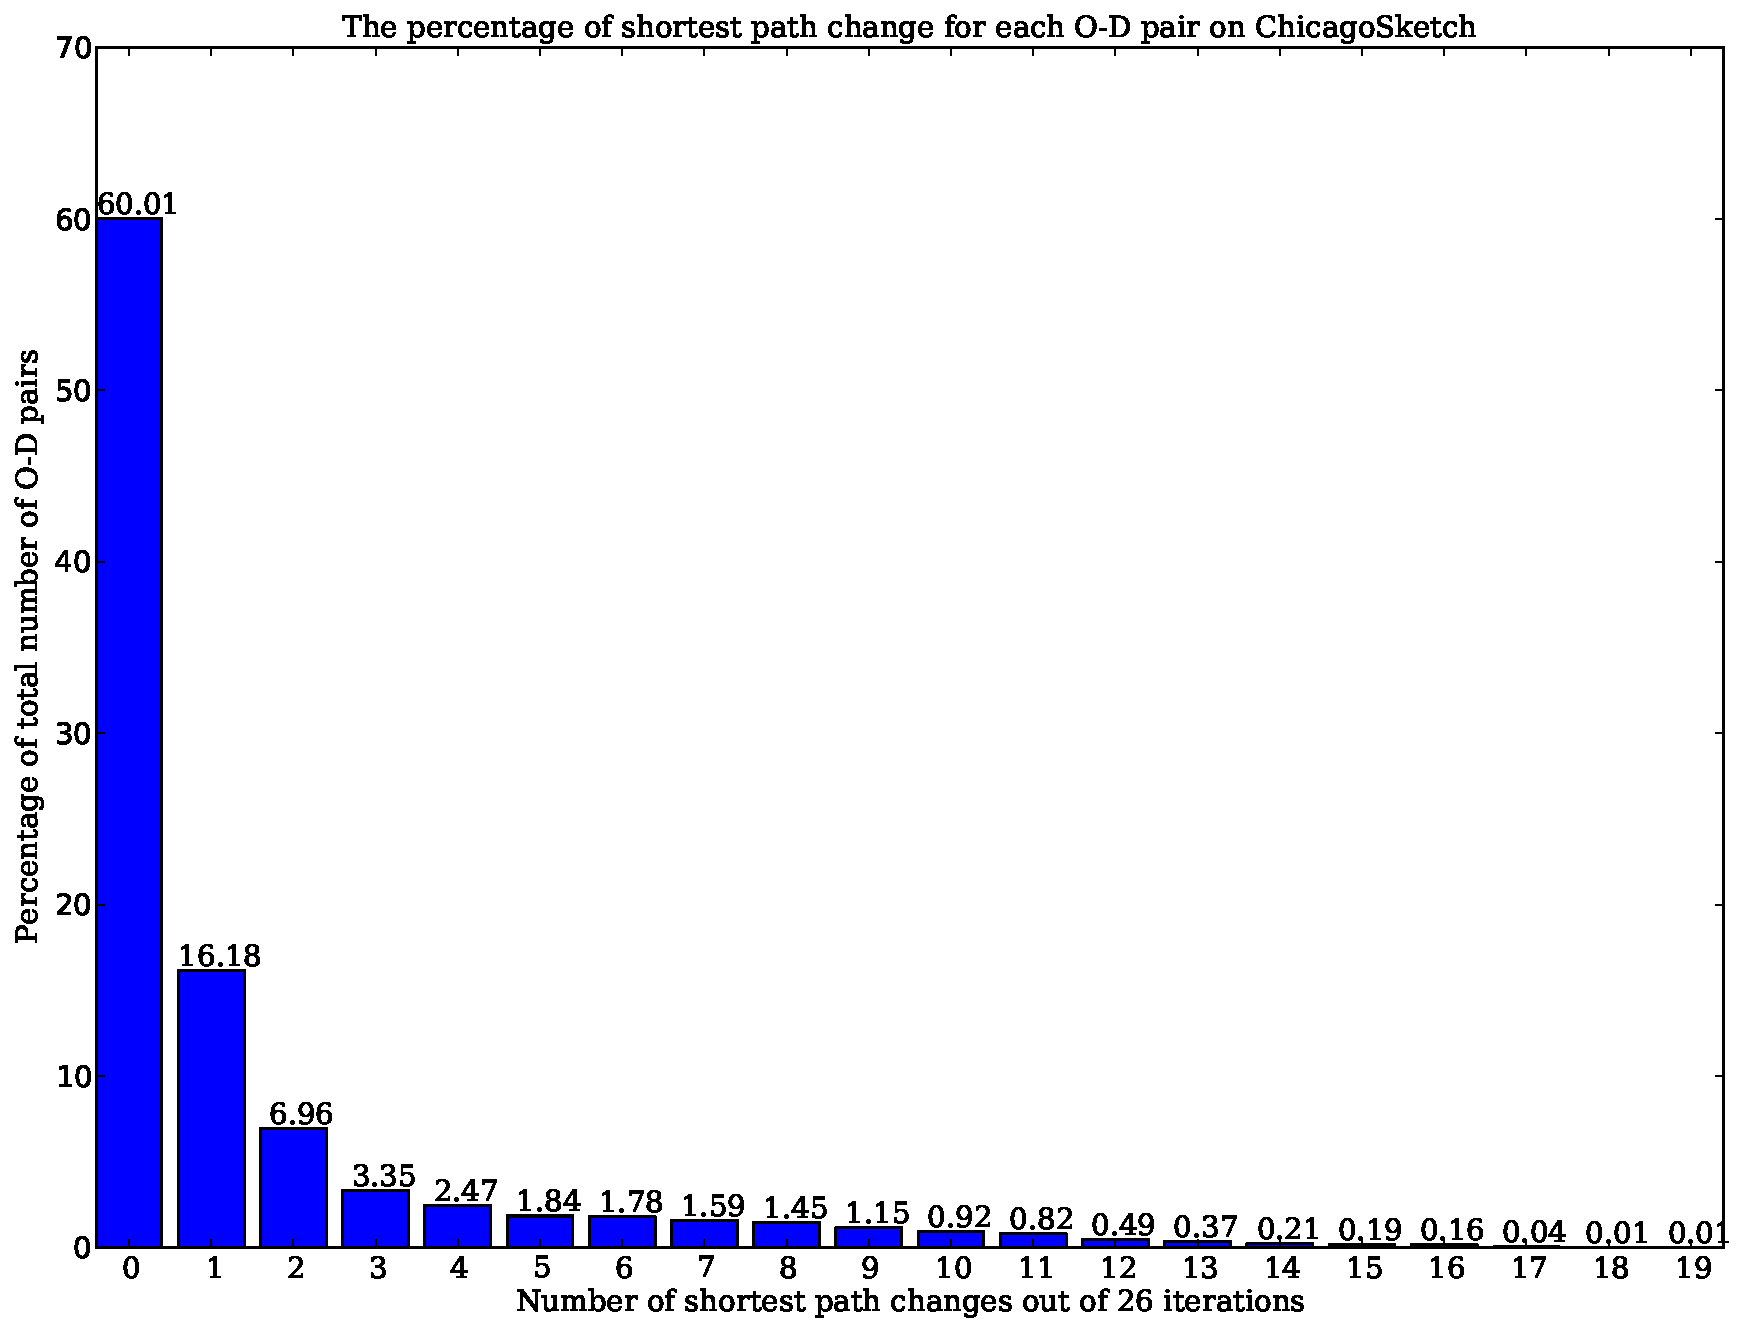
\includegraphics[width=\textwidth]{img/sp_change}
    \caption{The percentage of shortest path change for each O-D pair out of 26 iterations for ChicagoSketch}
    \label{fig:sp_change}
\end{figure}

\begin{figure}
    \centering
    \begin{subfigure}{.5\textwidth}
        \centering
        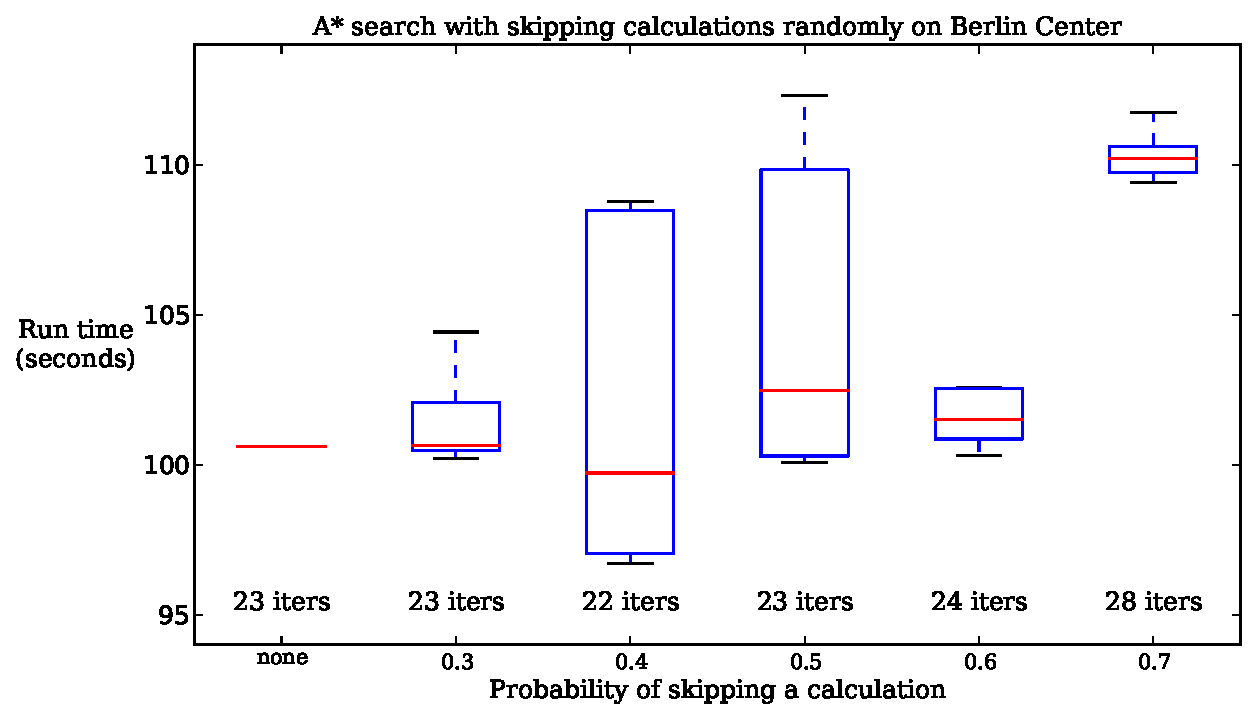
\includegraphics[page=1,width=\textwidth]{img/random_time}
        \caption{Terrassa network}
        \label{fig:terrassa_skip_n}
    \end{subfigure}%
    \begin{subfigure}{.5\textwidth}
        \centering
        \includegraphics[page=2,width=\textwidth]{img/random_time}
        \caption{ChicagoSketch network}
        \label{fig:chicago_skip_n}
    \end{subfigure}
    \caption{Run time for skipping shortest path calculations randomly}
    \label{fig:skip_n}
\end{figure}

\begin{figure}
    \centering
    \begin{subfigure}{.5\textwidth}
        \centering
        \includegraphics[page=3,width=\textwidth]{img/random_time}
        \caption{Terrassa network}
        \label{fig:terrassa_random_n}
    \end{subfigure}%
    \begin{subfigure}{.5\textwidth}
        \centering
        \includegraphics[page=4,width=\textwidth]{img/random_time}
        \caption{ChicagoSketch network}
        \label{fig:chicago_random_n}
    \end{subfigure}
    \caption{Run time for skipping shortest path calculations if the previous 2 did not change}
    \label{fig:random_n}
\end{figure}

